% ============================================================
% Chapter 5: The Vehicle Routing Problem with Time Windows
% Vehicle Routing: Problems, Methods, and Applications (2nd ed., 2014)
% Authors: Guy Desaulniers, Oli B.G. Madsen, Stefan Ropke
% Self-contained Beamer slides (reader-friendly, no presenter needed)
% ============================================================
\documentclass[aspectratio=169,10pt]{beamer}
\usetheme{Madrid}
\usecolortheme{seahorse}

\usepackage{amsmath,amssymb,amsfonts}
\usepackage{graphicx}
\usepackage{booktabs}
\usepackage{array}
\usepackage{xcolor}
\usepackage{listings}
\usepackage{algorithm}
\usepackage{algpseudocode}
\usepackage{tikz}
\usepackage{hyperref}
\usepackage{multirow}
\usepackage{microtype}

\graphicspath{{figures/}}

\lstset{
  language=Python,
  basicstyle=\ttfamily\scriptsize,
  numbers=left,
  numberstyle=\tiny\color{gray},
  frame=single,
  backgroundcolor=\color{gray!7},
  commentstyle=\color{green!50!black}\itshape,
  keywordstyle=\color{blue}\bfseries,
  stringstyle=\color{red!70!black},
  breaklines=true,
  showstringspaces=false,
  tabsize=4
}

\setbeamertemplate{footline}[frame number]
\setbeamertemplate{navigation symbols}{}

% ─── Title ──────────────────────────────────────────────────────────────────
\title[VRPTW]{The Vehicle Routing Problem with Time Windows}
\subtitle{Chapter 5 --- \textit{Vehicle Routing: Problems, Methods, and Applications}\\
  2nd Edition, 2014\\
  \small{Desaulniers, Madsen, Ropke}}
\author{Lecture Notes}
\date{2014}

% ============================================================
\begin{document}
% ============================================================

\begin{frame}
  \titlepage
\end{frame}

\begin{frame}[allowframebreaks]{Table of Contents}
  \tableofcontents
\end{frame}

% ============================================================
\section{Introduction}
% ============================================================

\begin{frame}[allowframebreaks]{What is the VRPTW?}

The \textbf{Vehicle Routing Problem with Time Windows (VRPTW)} is one of the most
studied and practically important variants of the classical Vehicle Routing Problem
(VRP).  In the standard VRP, a fleet of vehicles must deliver goods from a central
depot to a set of geographically dispersed customers, minimising total travel
distance or cost while respecting vehicle capacity limits.  The VRPTW adds a crucial
real-world constraint: each customer must be visited within a specified time interval
called a \emph{time window}.

\medskip
Consider a concrete example.  A grocery delivery service starts from a single
warehouse (the depot) and must deliver to 100 households.  Each household is only
available to receive the delivery between, say, 8\,am and 10\,am (a hard constraint
of two hours).  The planning problem is to assign deliveries to vehicles, sequence
them into routes, and ensure every household is served on time, while using as few
vehicles as possible and keeping total driving distance low.

\begin{figure}
  \centering
  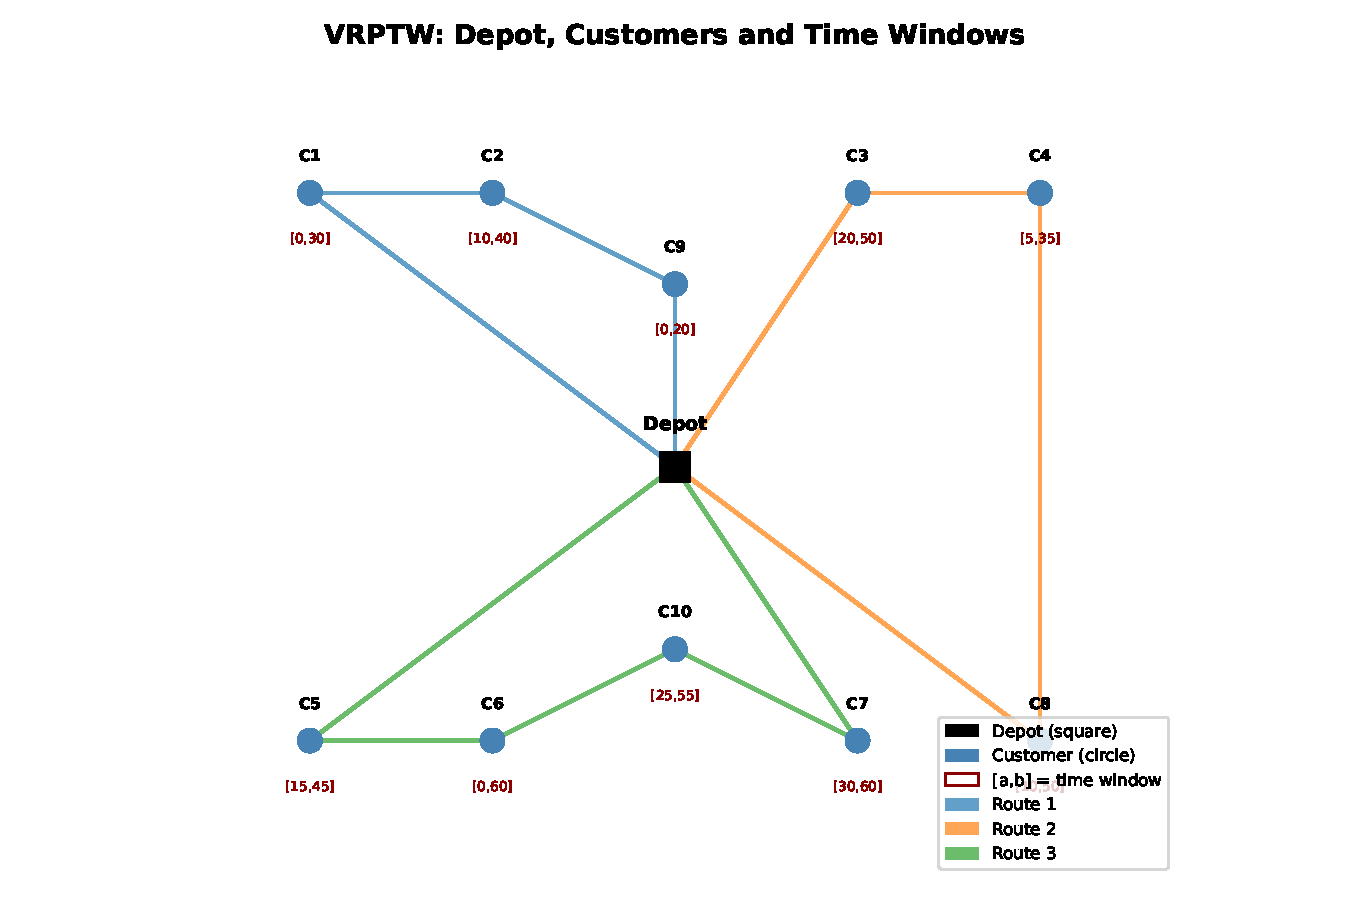
\includegraphics[width=0.72\textwidth]{vrptw_overview}
  \caption{A VRPTW instance with 10 customers and 3 vehicle routes.
    Each customer (blue circle) has a time window $[a_i, b_i]$ shown in red.
    Three colour-coded routes depart from and return to the depot (black square).}
\end{figure}

\framebreak

\begin{block}{Formal Problem Statement}
Given a complete directed graph $G = (V, A)$ where:
\begin{itemize}
  \item $V = \{0, 1, 2, \ldots, n, n+1\}$ is the set of nodes.  Nodes $0$ and
    $n+1$ both represent the depot (the starting and ending point); nodes $1$
    through $n$ represent customers.
  \item $A = \{(i,j) : i \neq j\}$ is the set of directed arcs (possible travel
    legs between any two locations).
  \item Each customer $i \in \{1,\ldots,n\}$ has a \emph{demand} $d_i$ (the
    quantity to be delivered), a \emph{time window} $[a_i, b_i]$ (earliest and
    latest permissible service start times), and a \emph{service time} $s_i$
    (time spent at the customer while unloading).
  \item Each arc $(i,j)$ has a \emph{travel time} $t_{ij}$ and a \emph{travel
    cost} $c_{ij}$ (often equal to the Euclidean distance between $i$ and $j$).
  \item A fleet of $m$ vehicles, each with capacity $Q$ (the maximum load it can
    carry), departs from and returns to the depot.
\end{itemize}
The goal is to find a set of routes---one per vehicle---such that (1) every
customer is visited exactly once, (2) each route starts and ends at the depot,
(3) vehicle capacity is never exceeded, (4) every customer is served within its
time window, and (5) total travel cost is minimised.
\end{block}

\end{frame}

\begin{frame}[allowframebreaks]{Why the VRPTW Matters}

The VRPTW is the canonical model for a vast range of logistics operations that
involve time-constrained delivery or service.  Among the most common real-world
applications are:

\begin{itemize}
  \item \textbf{Urban delivery and courier services:} Parcels must reach customers
    during the home-delivery window the customer selected at checkout.
  \item \textbf{Home health care:} Nurses or therapists visit patients who are only
    available at specific times and require a given duration of care.
  \item \textbf{School bus routing:} Students must be picked up and dropped off within
    legally defined windows around school start times.
  \item \textbf{Industrial waste collection:} Bins overflow if not emptied within
    specified periods; spillage constitutes a constraint violation.
  \item \textbf{Airport ground operations:} Aircraft servicing (refuelling, catering,
    cleaning) must complete before departure, creating tight time windows.
\end{itemize}

\begin{alertblock}{Key Insight}
The time-window constraint transforms the VRPTW from a pure
\emph{distance-minimisation} problem into a \emph{scheduling-and-routing}
problem.  Sequencing matters not just for distance but for feasibility:
inserting a customer with an early deadline in the wrong position can make
an otherwise short route infeasible.
\end{alertblock}

\framebreak

\textbf{Computational complexity.}  The classical VRP without time windows is already
NP-hard (it generalises the Travelling Salesman Problem).  Adding time windows
makes the problem even more constrained and, in the worst case, harder to solve.
However, tight time windows also \emph{prune} the search space significantly: many
sequences are immediately infeasible, and this structured infeasibility is exploited
by exact methods such as column generation.

\medskip
\textbf{Two objectives.}  In practice and in the literature, VRPTW solutions are
evaluated on two criteria, listed in order of priority:
\begin{enumerate}
  \item \textbf{Primary:} Minimise the total number of vehicles used.  Using fewer
    vehicles reduces fixed fleet costs.
  \item \textbf{Secondary:} Given the minimum number of vehicles, minimise the total
    travel distance or time.
\end{enumerate}
This hierarchical objective is why VRPTW algorithms report both the vehicle count and
the total distance of their best solutions.

\medskip
\textbf{Benchmark instances.}  Solomon (1987) introduced a widely used set of 56
benchmark instances with 100 customers each.  These instances are classified by the
spatial distribution of customers (random, clustered, or mixed) and by the width of
the time windows (tight or wide), yielding six classes: C1, C2, R1, R2, RC1, RC2.
Nearly all algorithmic comparisons in the VRPTW literature report results on these
instances.

\end{frame}

% ============================================================
\section{Mathematical Formulations}
% ============================================================

\begin{frame}[allowframebreaks]{5.2 --- Mathematical Formulations: Setup}

Before writing the mathematical model, we need to define all the variables and
parameters carefully.  This is important because the formulation guides both the
exact solution methods and the design of heuristics.

\begin{block}{Parameters and Sets}
\begin{itemize}
  \item $n$ \; --- number of customers (indexed $1$ to $n$).
  \item $V = \{0, 1, \ldots, n, n+1\}$ \; --- node set; $0$ and $n+1$ are the
    origin and destination depot copies.
  \item $V' = \{1, \ldots, n\}$ \; --- customer set (no depot).
  \item $K$ \; --- set of vehicles (indexed $1, \ldots, m$).
  \item $Q$ \; --- vehicle capacity (maximum load, in units of demand).
  \item $d_i$ \; --- demand of customer $i$ (units to deliver); $d_0 = d_{n+1} = 0$.
  \item $[a_i, b_i]$ \; --- time window for customer $i$; service must begin no
    earlier than $a_i$ (alpha sub $i$) and no later than $b_i$ (beta sub $i$).
  \item $s_i$ \; --- service time at customer $i$ (duration of unloading).
  \item $t_{ij}$ \; --- travel time from node $i$ to node $j$.
  \item $c_{ij}$ \; --- travel cost from node $i$ to node $j$ (often $= t_{ij}$
    when minimising time, or Euclidean distance when minimising distance).
\end{itemize}
\end{block}

\framebreak

\begin{block}{Decision Variables}
\begin{itemize}
  \item $x_{ij}^k$ \; --- binary variable equal to $1$ if vehicle $k$ travels
    directly from node $i$ to node $j$, and $0$ otherwise.  (Pronounced ``x
    sub $ij$ superscript $k$.'')
  \item $w_i^k$ \; --- continuous variable representing the time at which vehicle
    $k$ begins service at customer $i$.  (``w sub $i$ superscript $k$.'')
    If vehicle $k$ arrives before the time window opens, it must wait; if it
    arrives after $b_i$, the solution is infeasible.
\end{itemize}
\end{block}

\medskip
Note that $x_{ij}^k$ captures the \emph{routing} structure (which vehicle goes
where, in what order), while $w_i^k$ captures the \emph{timing} (when each service
starts).  These two families of variables are tightly linked: the timing $w_i^k$ is
determined by the sequence encoded in $x_{ij}^k$ together with travel and service
times.

\end{frame}

\begin{frame}[allowframebreaks]{5.2 --- The Three-Index VRPTW Formulation (Model I)}

The most transparent formulation uses three indices: one for the origin node $i$,
one for the destination node $j$, and one for the vehicle $k$.  This formulation is
sometimes called the \emph{vehicle-indexed arc formulation}.

\begin{block}{Objective Function (5.1)}
\[
  \min \sum_{k \in K} \sum_{(i,j) \in A} c_{ij} \, x_{ij}^k
\]
\end{block}

This objective function says: minimise the total travel cost summed over all arcs
$(i,j)$ in the network and all vehicles $k$.  Here $c_{ij}$ is the cost of
traversing arc $(i,j)$ (its distance or travel time), and $x_{ij}^k$ is the binary
indicator that vehicle $k$ uses that arc.  Only arcs actually used by a vehicle
contribute to the sum.

\begin{alertblock}{How to Read This}
Think of it this way: each vehicle ``draws'' a path on the map.  The total cost is
the sum of the distances of all arcs in all drawn paths.  We want the drawing to be
as short (cheap) as possible.  Adding more vehicles reduces each route's length but
adds fixed fleet costs (if modelled); in the pure VRPTW, the primary objective is
instead to minimise vehicle count, and distance is secondary.
\end{alertblock}

\framebreak

\begin{block}{Constraints}
\textbf{(5.2) Each customer is visited exactly once:}
\[
  \sum_{k \in K} \sum_{j \in V, j \neq i} x_{ij}^k = 1
  \qquad \forall\, i \in V'
\]
For each customer $i$, exactly one vehicle must travel the outgoing arc from $i$.
This ensures every customer is served by precisely one vehicle.

\medskip
\textbf{(5.3) Vehicles depart from the depot:}
\[
  \sum_{j \in V'} x_{0j}^k = 1
  \qquad \forall\, k \in K
\]
Each vehicle $k$ leaves the origin depot exactly once.  (Here we allow unused
vehicles too---in practice we may relax this to $\leq 1$.)

\medskip
\textbf{(5.4) Flow conservation at customer nodes:}
\[
  \sum_{i \in V} x_{ih}^k - \sum_{j \in V} x_{hj}^k = 0
  \qquad \forall\, h \in V',\; k \in K
\]
For each customer $h$ and each vehicle $k$: if vehicle $k$ arrives at $h$ (entering
arc $ih$), it must also depart from $h$ (outgoing arc $hj$).  This is the classic
\emph{flow conservation} constraint.  It prevents a vehicle from ``appearing'' or
``disappearing'' at a customer node.
\end{block}

\framebreak

\begin{block}{Constraints (continued)}
\textbf{(5.5) Vehicles return to the depot:}
\[
  \sum_{i \in V'} x_{i,n+1}^k = 1
  \qquad \forall\, k \in K
\]
Each vehicle returns to the destination depot copy ($n+1$) exactly once.

\medskip
\textbf{(5.6) Capacity constraint:}
\[
  \sum_{i \in V'} d_i \sum_{j \in V} x_{ij}^k \leq Q
  \qquad \forall\, k \in K
\]
The total demand delivered by vehicle $k$ must not exceed its capacity $Q$.
The inner sum $\sum_{j} x_{ij}^k$ counts whether customer $i$ is on vehicle $k$'s
route; if so, the demand $d_i$ contributes to the vehicle's load.

\medskip
\textbf{(5.7) Time window and timing consistency:}
\[
  x_{ij}^k = 1 \;\Rightarrow\; w_j^k \geq w_i^k + s_i + t_{ij}
  \qquad \forall\, (i,j) \in A,\; k \in K
\]
If vehicle $k$ travels arc $(i,j)$, then the service start time at $j$ must be at
least the service start time at $i$ plus the service duration $s_i$ at $i$ plus the
travel time $t_{ij}$ to $j$.  In other words, the vehicle cannot start serving $j$
before it has finished serving $i$ and driven from $i$ to $j$.

\medskip
\textbf{(5.8) Time window bounds:}
\[
  a_i \leq w_i^k \leq b_i
  \qquad \forall\, i \in V,\; k \in K
\]
Service at node $i$ by vehicle $k$ must begin within the time window $[a_i, b_i]$.

\medskip
\textbf{(5.9) Binary integrality:}
\[
  x_{ij}^k \in \{0, 1\}
  \qquad \forall\, (i,j) \in A,\; k \in K
\]
\end{block}

\framebreak

\begin{exampleblock}{Worked Example: 3 Customers, 2 Vehicles, Capacity $Q=10$}
Suppose we have 3 customers with demands $d_1=4$, $d_2=5$, $d_3=6$ and time windows
$[0,10]$, $[5,20]$, $[12,25]$, respectively.  Travel times: $t_{01}=2$, $t_{02}=3$,
$t_{03}=4$, $t_{12}=2$, $t_{13}=3$, $t_{23}=2$, and service times $s_i=1$ for all $i$.

\textbf{Candidate route for vehicle 1:} $0 \to 1 \to 2 \to n+1$.
\begin{itemize}
  \item Vehicle leaves depot at time 0.
  \item Arrives at customer 1 at time $t_{01}=2$; window $[0,10]$: start service
    at $w_1 = \max(2, a_1) = 2$.  Load so far: 4.
  \item Departs customer 1 at $2 + s_1 = 3$.  Arrives customer 2 at $3 + t_{12} = 5$.
    Window $[5,20]$: $w_2 = 5$.  Load: $4+5=9 \leq Q=10$. \checkmark
  \item Departs customer 2 at $5+1=6$.  Total load 9 $\leq$ 10. \checkmark
\end{itemize}

\textbf{Candidate route for vehicle 2:} $0 \to 3 \to n+1$.
\begin{itemize}
  \item Arrives customer 3 at $t_{03}=4$; window $[12,25]$: must wait until 12.
    $w_3 = 12$.  Load: 6 $\leq$ 10. \checkmark
\end{itemize}
Both routes are feasible.  The objective value is
$c_{01}+c_{12}+c_{2,n+1}+c_{03}+c_{3,n+1}$ (sum of arc costs).
\end{exampleblock}

\end{frame}

\begin{frame}[allowframebreaks]{5.2 --- Hard and Soft Time Windows}

The formulation above uses \emph{hard time windows}: late arrival is simply
infeasible (constraint 5.8 is inviolable).  Many real-world problems instead use
\emph{soft time windows}, where violations are penalised but allowed.

\begin{figure}
  \centering
  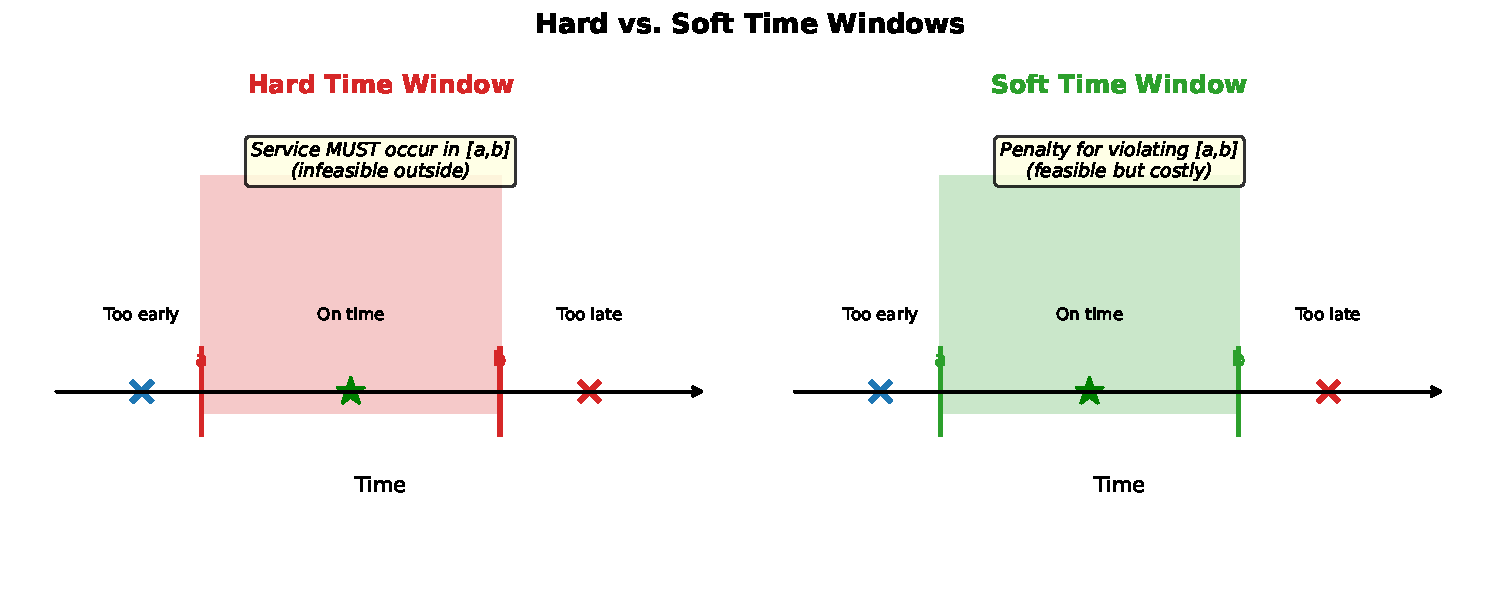
\includegraphics[width=0.78\textwidth]{hard_soft_tw}
  \caption{Left: Hard time window.  The vehicle must arrive in $[a,b]$; arriving
    outside this interval makes the solution infeasible.  Right: Soft time window.
    Arriving outside $[a,b]$ is allowed but incurs a penalty proportional to the
    violation amount.}
\end{figure}

\framebreak

\begin{block}{Soft Time Window Penalty}
For soft time windows, the objective function gains additional penalty terms.
A common formulation adds, for each customer $i$ and vehicle $k$:
\[
  \alpha_k^- \cdot \max(0,\; a_i - w_i^k) \;+\; \alpha_k^+ \cdot \max(0,\; w_i^k - b_i)
\]
Here $\alpha^-$ (alpha, the Greek letter for ``a'') is the penalty per unit of
\emph{early arrival} (the vehicle arrives before the window opens and must
wait---a possible cost if waiting is undesirable), and $\alpha^+$ is the penalty per
unit of \emph{late arrival} (the vehicle arrives after the window closes---a service
failure with a financial penalty or customer dissatisfaction cost).

The symbol $\max(0, \cdot)$ means we only take a positive value if the
violation is non-zero.  When $w_i^k \geq a_i$ (arrival on time or late), the early
penalty is zero; when $w_i^k \leq b_i$ (not late), the late penalty is zero.
\end{block}

\begin{alertblock}{Key Insight}
Hard time windows are the standard assumption in the VRPTW literature, because they
lead to cleaner formulations and allow meaningful comparison on Solomon benchmarks.
Soft time windows are more common in practice, especially in customer-facing
applications where a small lateness is tolerable at a known cost (e.g., a \$5
coupon for a late delivery).  The choice between hard and soft profoundly affects
which solution methods are applicable.
\end{alertblock}

\end{frame}

\begin{frame}[allowframebreaks]{5.2 --- The Two-Index Formulation (Model II)}

For many exact and heuristic methods, it is convenient to use a
\emph{vehicle-free} (two-index) formulation in which the vehicle index $k$ is
dropped.  This formulation is valid when all vehicles are homogeneous (identical
capacity and cost structure) and the objective is separable over arcs.

\begin{block}{Objective (5.10)}
\[
  \min \sum_{(i,j) \in A} c_{ij} \, x_{ij}
\]
where $x_{ij} \in \{0,1\}$ indicates whether arc $(i,j)$ is used by \emph{any}
vehicle (we no longer track which specific vehicle uses it).
\end{block}

\begin{block}{Key Constraints}
\textbf{(5.11) Each customer visited once:}
\[
  \sum_{j \in V \setminus \{i\}} x_{ij} = 1 \qquad \forall\, i \in V'
\]

\textbf{(5.12) Flow conservation:}
\[
  \sum_{i \in V} x_{ij} = \sum_{i \in V} x_{ji} \qquad \forall\, j \in V'
\]

\textbf{(5.13) Timing consistency} (linearised):
\[
  w_j \geq w_i + s_i + t_{ij} - M(1 - x_{ij}) \qquad \forall\, (i,j) \in A
\]
Here $M$ (a large number, called the ``big-M'') is a sufficiently large constant
that when $x_{ij}=0$, the constraint is trivially satisfied.  When $x_{ij}=1$, it
enforces the timing logic: $w_j \geq w_i + s_i + t_{ij}$.
\end{block}

\framebreak

\begin{alertblock}{Two-Index vs.\ Three-Index: Trade-offs}
The three-index formulation (Model I) has $O(n^2 m)$ binary variables and $O(n^2 m)$
constraints.  For large instances with many vehicles, this is huge.  The two-index
formulation has $O(n^2)$ binary variables but loses the ability to enforce
vehicle-specific constraints (e.g., different capacities per vehicle).  In practice,
the \emph{set-partitioning} formulation described next is often preferred for exact
methods because its LP relaxation is much tighter.
\end{alertblock}

\begin{block}{Number of Vehicles}
The minimum number of vehicles is sometimes enforced as a lower bound constraint.
If we want at most $m$ vehicles:
\[
  \sum_{j \in V'} x_{0j} \leq m
\]
This is the constraint that ``at most $m$ routes depart from the depot.''  In
hierarchical VRPTW, vehicle minimisation is the \emph{primary} objective, so one
first solves for the minimum number of vehicles and then minimises distance with
that fixed fleet size.
\end{block}

\end{frame}

\begin{frame}[allowframebreaks]{5.2 --- Set Partitioning Formulation (Model III)}

The \emph{set partitioning} (or \emph{path-based}) formulation is the foundation of
the most powerful exact algorithms.  Instead of modelling individual arcs, it
operates over the set of all feasible routes.

\begin{block}{Set-Partitioning Model}
Let $\mathcal{R}$ be the set of all feasible routes (paths from depot $0$ to depot
$n+1$ that respect capacity and time windows).  For each route $r \in \mathcal{R}$:
\begin{itemize}
  \item $c_r$ \; --- total travel cost of route $r$.
  \item $a_{ir} \in \{0,1\}$ \; --- equals 1 if customer $i$ appears on route $r$,
    and 0 otherwise.
  \item $\lambda_r$ (lambda sub $r$, the Greek letter lambda) \; --- binary
    decision variable equal to 1 if route $r$ is selected in the solution.
\end{itemize}

\textbf{Objective:}
\[
  \min \sum_{r \in \mathcal{R}} c_r \, \lambda_r
\]
\textbf{Coverage constraints (each customer served exactly once):}
\[
  \sum_{r \in \mathcal{R}} a_{ir} \, \lambda_r = 1 \qquad \forall\, i \in V'
\]
\textbf{Integrality:}
\[
  \lambda_r \in \{0, 1\} \qquad \forall\, r \in \mathcal{R}
\]
\end{block}

\framebreak

\begin{alertblock}{Why the Set-Partitioning Formulation?}
The LP relaxation (where $\lambda_r \in [0,1]$ instead of $\{0,1\}$) of the
set-partitioning model is \emph{much tighter} (closer to the optimal integer
value) than the LP relaxation of the arc-based formulations.  This means that
Branch-and-Bound algorithms need far fewer nodes to prove optimality.  The downside
is that $|\mathcal{R}|$ is exponentially large, so the formulation cannot be solved
directly.  Instead, \textbf{column generation} is used to implicitly enumerate only
the routes needed to describe the optimal solution.
\end{alertblock}

\begin{exampleblock}{Worked Example: Set Partitioning with 3 Customers}
Suppose 3 customers and the feasible routes are:
$r_1 = \{1,2\}$, $r_2 = \{3\}$, $r_3 = \{1\}$, $r_4 = \{2,3\}$, with costs
$c_1=10$, $c_2=6$, $c_3=7$, $c_4=9$.

\medskip
Coverage constraints:
\begin{align*}
  &\lambda_1 + \lambda_3 = 1 \quad (\text{customer 1 served by } r_1 \text{ or } r_3)\\
  &\lambda_1 + \lambda_4 = 1 \quad (\text{customer 2 served by } r_1 \text{ or } r_4)\\
  &\lambda_2 + \lambda_4 = 1 \quad (\text{customer 3 served by } r_2 \text{ or } r_4)
\end{align*}
Optimal solution: $\lambda_1 = 1, \lambda_2 = 1$ (routes $r_1$ and $r_2$),
cost $= 10 + 6 = 16$.  Alternatively $\lambda_3=1, \lambda_4=1$, cost $= 7+9=16$.
Both use 2 vehicles and cost 16.
\end{exampleblock}

\end{frame}

% ============================================================
\section{Exact Solution Methods}
% ============================================================

\begin{frame}[allowframebreaks]{5.3 --- Exact Methods: Overview}

Because the VRPTW is NP-hard, exact methods can only solve instances of limited
size (up to around 100 customers in practice, with great difficulty).  Nevertheless,
exact methods are important because they (a) prove optimal solutions for benchmark
instances, establishing reference points; (b) provide lower bounds for heuristic
quality; and (c) generate structural insights that inform heuristic design.

\medskip
The main exact approaches for the VRPTW are:

\begin{enumerate}
  \item \textbf{Branch-and-Bound with arc-based LP relaxation.}  An early approach
    that solves the LP relaxation at each node of a branch-and-bound tree.  The LP
    relaxation is weak, so many nodes are needed.

  \item \textbf{Column generation} (solving the LP relaxation of the set-partitioning
    formulation).  This is the foundation of modern exact methods.  Instead of
    enumerating all routes, it dynamically generates only the routes with potential
    to improve the solution.

  \item \textbf{Branch-and-Price} (B\&P).  Combines branch-and-bound with column
    generation at each node.  This is the \emph{state-of-the-art} exact approach
    and can solve instances with up to about 100 customers.

  \item \textbf{Branch-and-Price-and-Cut} (B\&P\&C).  Adds cutting planes to
    tighten the LP relaxation, further reducing the tree size.
\end{enumerate}

\end{frame}

\begin{frame}[allowframebreaks]{5.3.1 --- Column Generation}

Column generation is the key technique that makes it tractable to solve the LP
relaxation of the set-partitioning formulation.  The core idea is: instead of
including all exponentially many routes in the LP from the start, begin with a small
\emph{initial set} of routes (columns) and iteratively \emph{add} only routes that
can improve the current LP solution.

\begin{block}{The Column Generation Loop}
\begin{enumerate}
  \item \textbf{Solve the Restricted Master Problem (RMP):} Solve the LP relaxation
    with the current set of columns (routes).  Obtain dual variables
    $\pi_i$ (pi sub $i$, Greek letter pi) for each customer $i$'s coverage
    constraint.

  \item \textbf{Solve the Pricing Sub-problem:} Find a feasible route $r$ with
    \emph{negative reduced cost}:
    \[
      \bar{c}_r = c_r - \sum_{i \in r} \pi_i < 0
    \]
    Here $\bar{c}_r$ (c-bar sub $r$) is the reduced cost.  The term $c_r$ is the
    route's travel cost; the term $\sum_{i \in r} \pi_i$ is the ``value'' of the
    customers on that route according to the current dual prices $\pi_i$.

  \item \textbf{Add column:} If such a route is found, add it to the RMP and
    return to step 1.

  \item \textbf{Optimality certificate:} If no route with negative reduced cost
    exists, the current RMP solution is the optimal LP solution.
\end{enumerate}
\end{block}

\framebreak

\begin{alertblock}{How to Read the Reduced Cost Formula}
The reduced cost $\bar{c}_r = c_r - \sum_{i \in r} \pi_i$ measures whether adding
route $r$ to the solution can reduce the total objective.  The dual variable
$\pi_i$ represents the ``shadow price'' of serving customer $i$: how much the
objective would change if customer $i$'s coverage requirement were relaxed.  A route
with $\bar{c}_r < 0$ means its cost is \emph{less} than the combined value of serving
its customers---so including it is beneficial.

\medskip
Intuitively: if the LP is currently paying a lot to serve customer $i$ (high $\pi_i$),
then any route that cheaply includes $i$ has a negative reduced cost and should be
considered.
\end{alertblock}

\begin{figure}
  \centering
  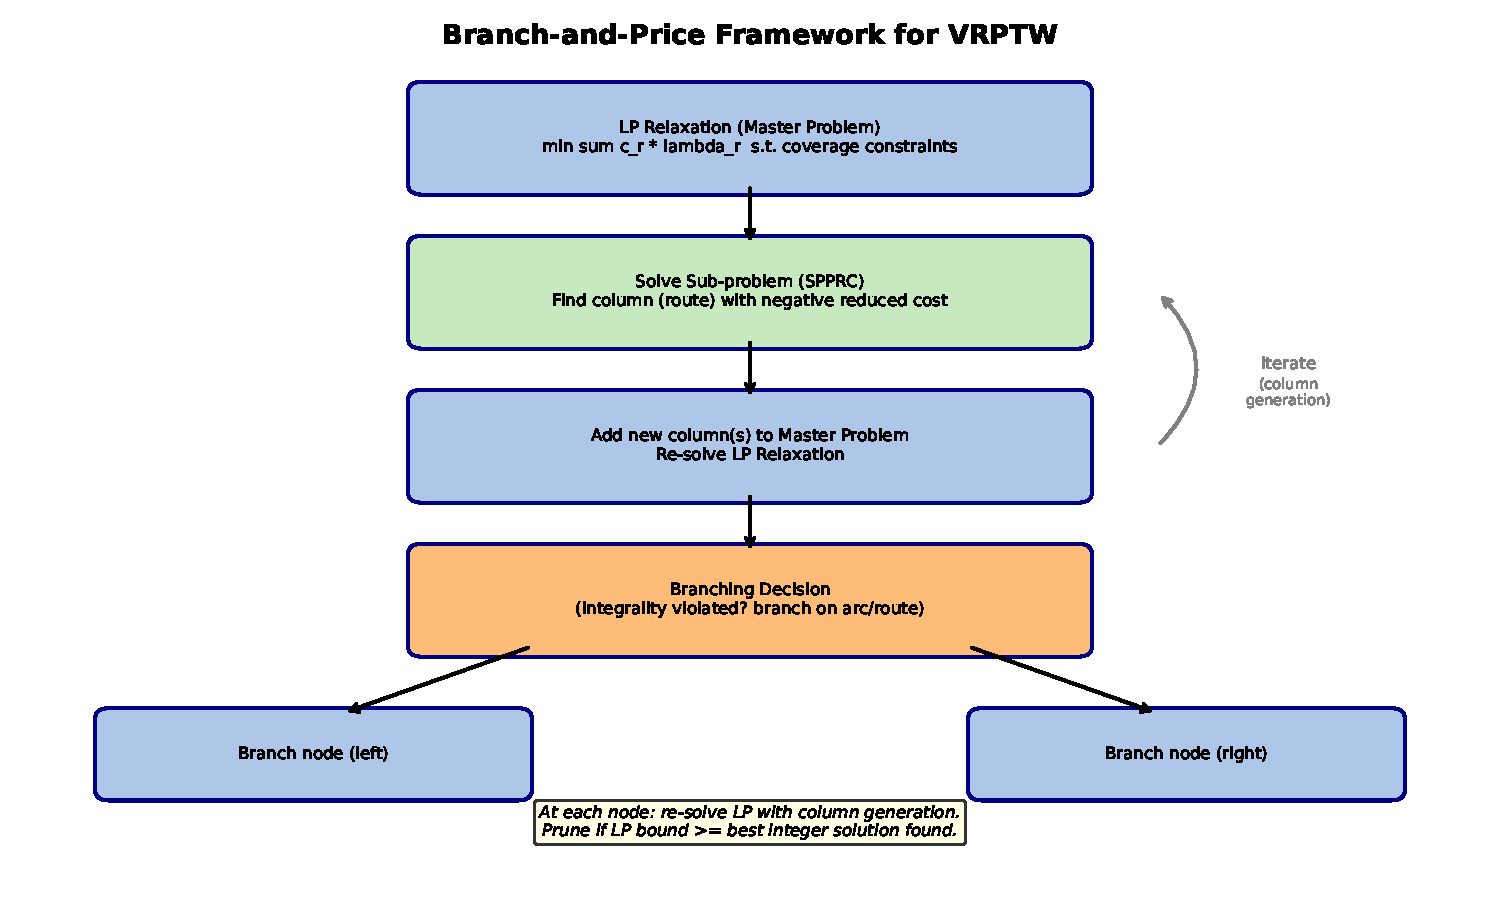
\includegraphics[width=0.70\textwidth]{branch_price}
  \caption{The Branch-and-Price framework.  Column generation solves the LP
    relaxation at each branch-and-bound node.  When the LP is optimal, a branching
    decision is made on a fractional variable.}
\end{figure}

\framebreak

\begin{figure}
  \centering
  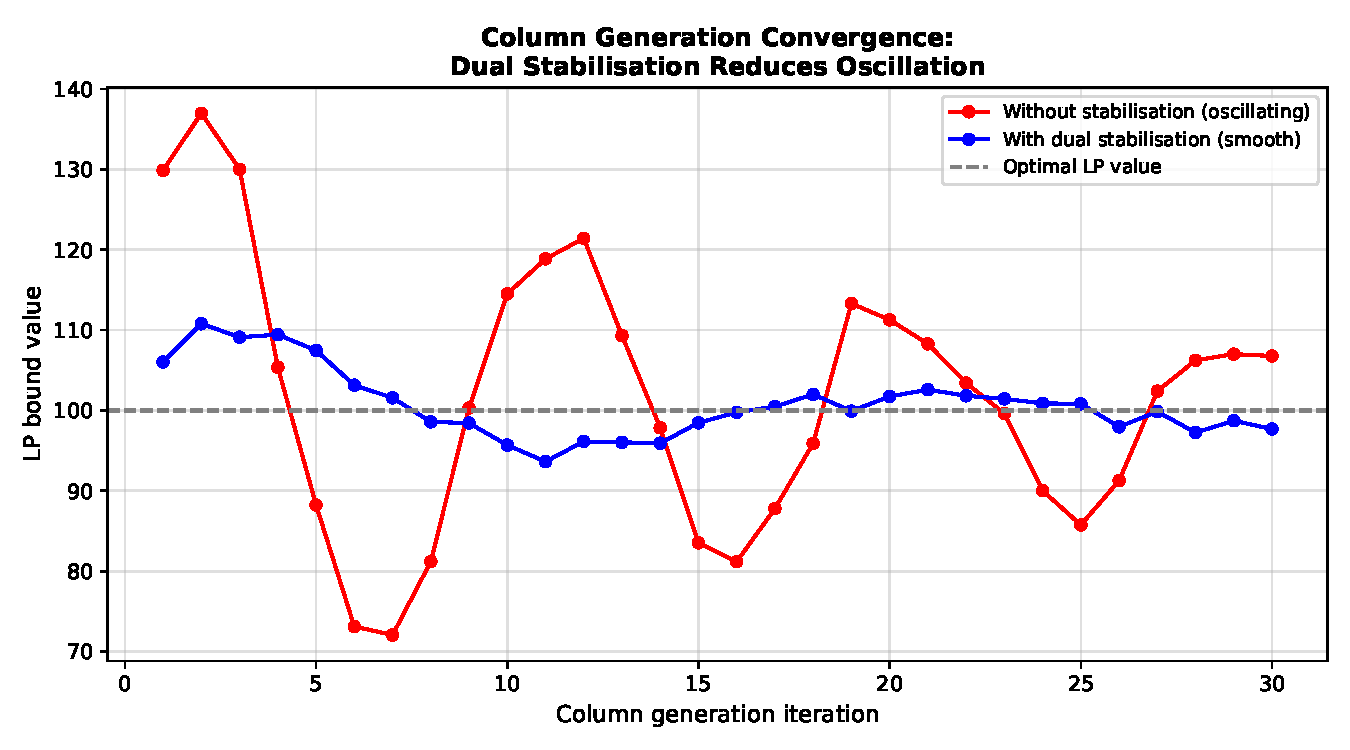
\includegraphics[width=0.72\textwidth]{cg_convergence}
  \caption{Column generation convergence.  Without dual stabilisation (red), the LP
    bound oscillates because dual variables swing wildly between iterations.  With
    stabilisation techniques such as bundle methods or proximal-point terms (blue),
    convergence is smoother and faster.}
\end{figure}

\textbf{Dual stabilisation.}  A known practical difficulty with column generation is
that dual variables can oscillate severely between iterations, especially early in
the process.  This slows convergence dramatically.  Stabilisation methods---such as
adding a \emph{proximal term} to the RMP objective or restricting dual variables to
a box around their current values---damp these oscillations and accelerate
convergence.  Dual stabilisation was introduced for the VRPTW by Rousseau,
Gendreau, and Feillet (2007).

\end{frame}

\begin{frame}[allowframebreaks]{5.3.1 --- The Pricing Sub-problem: SPPRC}

The pricing sub-problem---finding a feasible route with minimum reduced cost---is
itself a non-trivial combinatorial problem.  For the VRPTW, it is formulated as the
\textbf{Shortest Path Problem with Resource Constraints (SPPRC)}.

\begin{block}{SPPRC: What Problem Does It Solve?}
We seek the least-cost path from the origin depot (node 0) to the destination
depot (node $n+1$) in the network $G$, where the path must satisfy two
\emph{resource} constraints at every intermediate node:
\begin{enumerate}
  \item \textbf{Time resource:} The earliest feasible service start time at each
    node must fall within the node's time window $[a_i, b_i]$.
  \item \textbf{Load resource:} The cumulative demand picked up along the path
    must not exceed the vehicle capacity $Q$.
\end{enumerate}
The ``cost'' of an arc $(i,j)$ in the pricing sub-problem is its \emph{reduced
travel cost} $c_{ij} - \pi_j$ (since the reduced cost of including node $j$ on
the route reduces the route's reduced cost by $\pi_j$).
\end{block}

\framebreak

\begin{block}{Resource Extension Functions}
The SPPRC is solved via \emph{dynamic programming over labels}.  A label at node
$j$ is a tuple $(T_j, Q_j)$ where:
\begin{itemize}
  \item $T_j$ is the earliest feasible time at which the vehicle can start serving
    customer $j$ (respecting earlier time windows on the path so far).
  \item $Q_j$ is the total demand of customers visited so far on the path.
\end{itemize}
When extending a path from node $i$ to node $j$, the label is updated by the
\emph{resource extension functions} (REFs):
\[
  T_j = \max\bigl(T_i + s_i + t_{ij},\; a_j\bigr)
  \qquad
  Q_j = Q_i + d_j
\]
The first equation says: the earliest arrival time at $j$ is the current time
($T_i$) plus service time at $i$ ($s_i$) plus travel time from $i$ to $j$
($t_{ij}$), but if we arrive before the window opens, we must wait until $a_j$.
The second equation simply adds the demand of customer $j$.

\medskip
A label is \emph{infeasible} if $T_j > b_j$ (late arrival) or $Q_j > Q$
(capacity exceeded); such labels are discarded.
\end{block}

\begin{figure}
  \centering
  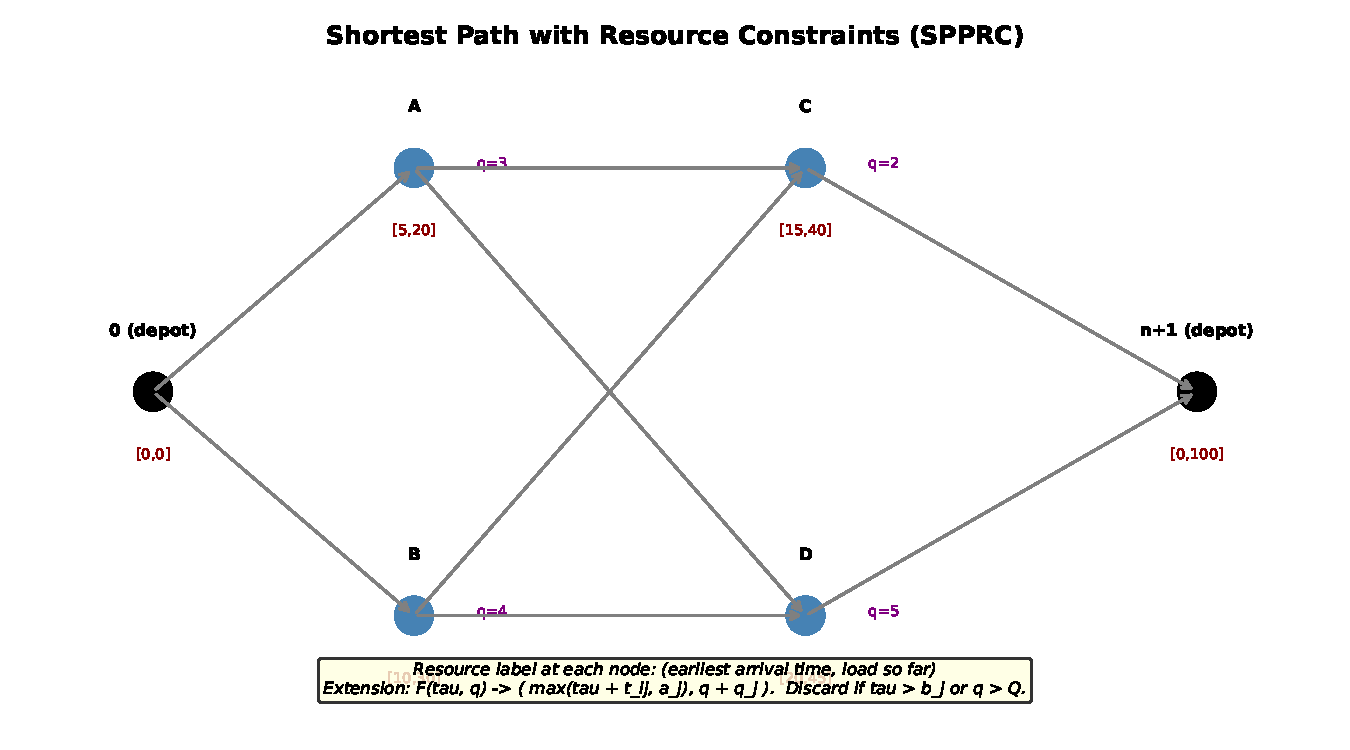
\includegraphics[width=0.72\textwidth]{spprc}
  \caption{SPPRC on a small network.  The depot (node 0) and destination depot
    (node $n+1$) are shown in black; customers A, B, C, D are shown in blue.
    Each node has a time window (red) and demand (purple).  Dynamic programming
    propagates resource labels along arcs, pruning infeasible extensions.}
\end{figure}

\framebreak

\begin{block}{Label Dominance (Pruning)}
To avoid an exponential blowup in labels, we apply \emph{dominance}: label
$L_1 = (T_1, Q_1)$ \emph{dominates} label $L_2 = (T_2, Q_2)$ at the same node if
\[
  T_1 \leq T_2 \quad \text{and} \quad Q_1 \leq Q_2
\]
This means $L_1$ is at least as good as $L_2$ on \emph{both} resources.  Any
extension of $L_2$ could also be achieved (and at least as well) by extending $L_1$.
Therefore $L_2$ can be discarded without losing optimality.

\medskip
With dominance pruning, the labelling algorithm runs in pseudo-polynomial time.
For each node $j$, we maintain only the set of \emph{non-dominated} labels (the
Pareto front of labels in $(T,Q)$ space).
\end{block}

\begin{block}{Complexity Note}
The SPPRC with time windows and capacity is NP-hard in general (it is equivalent
to solving a constrained shortest path, which is NP-hard when there are two or more
resources).  However, the tight time windows in VRPTW instances severely restrict
the number of non-dominated labels at each node, making the labelling algorithm
tractable in practice.  Proposition 1 (Desaulniers et al.) states that in
bi-directional labelling, the two-label representation suffices.
\end{block}

\end{frame}

\begin{frame}[allowframebreaks]{5.3.1 --- Labelling Algorithm for SPPRC}

The labelling algorithm is a generalisation of Dijkstra's algorithm that tracks
resource consumption along each path.

\begin{algorithm}[H]
\caption{Forward Labelling Algorithm for SPPRC}
\begin{algorithmic}[1]
\State Initialise: at node $0$ (depot), create label $L_0 = (T=0, Q=0, \text{cost}=0)$.
\State Mark all nodes unprocessed.  Add $L_0$ to the label set of node 0.
\While{there exists an unprocessed label}
  \State Select an unprocessed label $L = (T_i, Q_i)$ at node $i$ with minimum cost.
  \State Mark $L$ as processed.
  \For{each arc $(i,j) \in A$}
    \State Compute extended label: $T_j \leftarrow \max(T_i + s_i + t_{ij},\; a_j)$
    \State $Q_j \leftarrow Q_i + d_j$
    \If{$T_j \leq b_j$ \textbf{and} $Q_j \leq Q$}
      \State Create new label $L' = (T_j, Q_j, \text{cost}_L + \bar{c}_{ij})$
      \If{$L'$ is not dominated by any label at $j$}
        \State Add $L'$ to label set of $j$; remove dominated labels.
      \EndIf
    \EndIf
  \EndFor
\EndWhile
\State \Return label at node $n+1$ with minimum cost (= minimum reduced cost route).
\end{algorithmic}
\end{algorithm}

\textbf{Step-by-step explanation:}
\begin{itemize}
  \item \textbf{Line 1:} We start at the depot with zero time elapsed, zero load,
    and zero cost accumulated.
  \item \textbf{Lines 5--7:} For each possible next customer $j$, we compute the
    earliest time we can start serving $j$ given that we have just finished at $i$.
    The $\max(\cdot, a_j)$ ensures we wait if we arrive before the window opens.
  \item \textbf{Lines 8--9:} We check feasibility: did we arrive before the deadline
    ($T_j \leq b_j$) and is the vehicle still within capacity ($Q_j \leq Q$)?
  \item \textbf{Lines 10--12:} Only keep the new label if it is not dominated by
    another label already at node $j$ (dominance pruning).
  \item \textbf{Line 13:} The best label reaching the destination depot is the
    negative-reduced-cost route to add to the master problem.
\end{itemize}

\end{frame}

\begin{frame}[allowframebreaks]{5.3.2 --- Branch-and-Price}

Column generation solves the LP relaxation of the set-partitioning formulation.
To obtain an integer (combinatorial) solution, we embed column generation inside a
\textbf{branch-and-bound} framework.  The combination is called
\textbf{Branch-and-Price (B\&P)}.

\begin{block}{Why Not Just Round the LP Solution?}
The LP relaxation of the set-partitioning model allows $\lambda_r$ to be fractional
(e.g., $\lambda_r = 0.5$, meaning half a route).  Rounding these values up or down
typically produces infeasible or heavily suboptimal solutions.  The branch-and-bound
tree systematically explores all integer solutions implied by the LP relaxation,
pruning branches that cannot improve on the best integer solution found so far.
\end{block}

\begin{block}{Branching Strategies for VRPTW}
Standard branching on LP variables ($\lambda_r = 0$ or $1$) destroys the pricing
sub-problem structure.  Instead, two branching strategies are commonly used:

\begin{enumerate}
  \item \textbf{Branch on arc flow:} Force arc $(i,j)$ to be used (or not) by at
    least one vehicle.  Formally: $\sum_{r: (i,j) \in r} \lambda_r \geq 1$ or $= 0$.
    This modifies the SPPRC by forbidding or requiring specific arcs.

  \item \textbf{Branch on the number of vehicles serving a cluster:} Group customers
    into a cluster and branch on whether the number of vehicles serving that cluster
    is $\leq k$ or $\geq k+1$.
\end{enumerate}

The most popular strategy (Desrochers, Desrosiers, and Solomon 1992) branches on
arc flow, which can be imposed directly in the SPPRC by removing or requiring arcs.
\end{block}

\framebreak

\begin{block}{Valid Inequalities to Strengthen the Formulation}
Various cutting planes can be added to tighten the LP relaxation at each B\&P node:

\begin{itemize}
  \item \textbf{Infeasible path inequalities:} Forbid sequences of arcs that are
    jointly infeasible due to time windows.  For a sequence $S = (i_1, i_2, i_3)$
    where visiting all three in order is time-infeasible, add:
    \[
      \sum_{r: S \subseteq r} \lambda_r = 0
    \]

  \item \textbf{$k$-path cuts (subset-row inequalities):} For any subset
    $S \subseteq V'$ of customers, the minimum number of routes needed to cover
    $S$ provides a lower bound on the number of routes intersecting $S$:
    \[
      \sum_{r \in \mathcal{R}} \lfloor |r \cap S| / 2 \rfloor \cdot \lambda_r
      \leq |K|
    \]
    (where $|K|$ is the fleet size).  These cuts are called \emph{subset-row
    inequalities} (SRIs) or $k$-path cuts and significantly tighten the LP.

  \item \textbf{Capacity cuts:} Standard Gomory-Hu capacity inequalities from
    the VRP.
\end{itemize}
\end{block}

\begin{alertblock}{State of the Art}
The Branch-and-Price-and-Cut algorithm of Chabrier (2006) and the bidirectional
SPPRC labelling of Righini and Salani (2006, 2008) pushed the frontier to instances
of 100 customers.  For instances beyond 100 customers, exact methods remain too slow
and heuristic methods are necessary.
\end{alertblock}

\end{frame}

\begin{frame}[allowframebreaks]{5.3.3 --- Reduced Cost Variable Fixing}

An important technique to speed up Branch-and-Price is \emph{reduced cost variable
fixing} (also called \emph{reduced cost pricing}).  The idea is to eliminate arcs or
routes from consideration \emph{before} solving the full pricing sub-problem, by
exploiting the current LP dual solution.

\begin{block}{Principle}
Suppose the current LP optimal value is $z^*_{LP}$ and the best known integer
solution has value $\bar{z}$.  For any arc $(i,j)$, define its reduced cost as:
\[
  \bar{c}_{ij} = c_{ij} - \pi_i - \mu_j
\]
where $\pi_i$ (pi sub $i$) and $\mu_j$ (mu sub $j$, Greek letter mu) are dual
variables.  If $z^*_{LP} + \bar{c}_{ij} > \bar{z}$, then using arc $(i,j)$ in any
route cannot improve the integer solution.  Such arcs can be \emph{fixed to zero}
(removed from the network), reducing the SPPRC complexity.

\medskip
In practice, reduced cost fixing can eliminate 50--90\% of arcs in tight instances,
dramatically accelerating the pricing sub-problem.
\end{block}

\end{frame}

% ============================================================
\section{Heuristics}
% ============================================================

\begin{frame}[allowframebreaks]{5.4 --- Heuristics: Overview and Motivation}

Exact methods for the VRPTW become computationally intractable for large instances
(more than 100--150 customers).  Real-world logistics instances regularly involve
hundreds to thousands of customers.  \textbf{Heuristics} sacrifice the guarantee of
finding the optimal solution in exchange for finding high-quality solutions quickly.

\medskip
The heuristic landscape for VRPTW divides naturally into three levels:

\begin{enumerate}
  \item \textbf{Construction heuristics:} Build a feasible solution from scratch.
    They do not improve an existing solution; they produce a starting point.
    Examples: Solomon's insertion algorithms I1 and I2 (1987).

  \item \textbf{Local search and improvement heuristics:} Start from a feasible
    solution and iteratively improve it by making small modifications
    (\emph{moves}).  Examples: 2-opt, Or-opt, cross-exchange.  They are fast but
    can get trapped in local optima.

  \item \textbf{Metaheuristics:} Higher-level frameworks that guide local search to
    escape local optima.  Examples: Tabu Search, Simulated Annealing, Genetic
    Algorithms, Large Neighbourhood Search.  These are the methods that achieve
    best-known solutions on Solomon benchmarks.
\end{enumerate}

\end{frame}

\begin{frame}[allowframebreaks]{5.4.1 --- Solomon's Insertion Heuristics (I1, I2)}

Solomon (1987) proposed the first systematic construction heuristics for the VRPTW.
The most important is the \textbf{I1 algorithm}: a sequential insertion procedure
that builds one route at a time and inserts customers based on a scoring function
that balances distance and time window proximity.

\medskip
\textbf{Intuition.}  Starting from an empty route (just the depot), we repeatedly
ask: which unrouted customer, if inserted at the best feasible position in the
current route, causes the least additional cost?  We insert that customer, update
the route's timing, and repeat until no more customers can be feasibly inserted.
Then we open a new route for the remaining customers.

\begin{block}{I1 Algorithm: Criterion Functions}
For inserting customer $u$ between currently consecutive customers $i$ and $j$ on
the route:

\textbf{Cost criterion} $c_1(i, u, j)$: the extra distance caused by the insertion:
\[
  c_1(i, u, j) = \alpha_1 \cdot (d_{iu} + d_{uj} - d_{ij})
              + \alpha_2 \cdot b_u^* - b_j^*
\]
Here $d_{ij}$ (d sub $ij$) is the distance between $i$ and $j$;
$b_u^*$ (b-star sub $u$) is the new service start time at $u$ if inserted;
$b_j^*$ (b-star sub $j$) is the resulting new service start time at $j$ after
the insertion.  The parameters $\alpha_1$ (alpha sub 1) and $\alpha_2$ (alpha sub 2)
weight the distance increase against the time-push effect (how much the insertion
delays later customers).  Typically $\alpha_1 + \alpha_2 = 1$.
\end{block}

\framebreak

\begin{block}{I1 Algorithm: Selection Criterion}
\textbf{Selection criterion} $c_2(u)$: which unrouted customer $u$ to insert.
The best position for $u$ is the one that minimises $c_1$; call this minimum cost
$c_1^*(u)$.  Among all unrouted customers, we select the one with maximum
\[
  c_2(u) = \lambda \cdot d(depot, u) - c_1^*(u)
\]
Here $\lambda$ (lambda) is a parameter.  The term $d(depot, u)$ is the distance
from the depot to customer $u$; subtracting the best insertion cost $c_1^*(u)$
biases selection toward customers that are \emph{far from the depot but cheap to
insert}---these are the customers who would be most expensive to handle in a future
route if not inserted now.
\end{block}

\begin{block}{I1 Algorithm: Pseudocode}
\begin{algorithmic}[1]
\State $\mathcal{U} \leftarrow \{1,\ldots,n\}$ (all customers unrouted)
\While{$\mathcal{U} \neq \emptyset$}
  \State Select seed customer: $u_0 \leftarrow \arg\max_{u \in \mathcal{U}} d(depot, u)$
    (or earliest deadline)
  \State Create new route: $R \leftarrow (depot \to u_0 \to depot)$;
    $\mathcal{U} \leftarrow \mathcal{U} \setminus \{u_0\}$
  \Repeat
    \For{each $u \in \mathcal{U}$}
      \State Find best feasible insertion position $(i^*, j^*)$ in $R$ minimising
        $c_1(i, u, j)$
    \EndFor
    \If{any feasible insertion exists}
      \State Insert $u^* = \arg\max c_2(u)$ at position $(i^*, j^*)$;
        $\mathcal{U} \leftarrow \mathcal{U} \setminus \{u^*\}$
    \EndIf
  \Until{no feasible insertion exists or $\mathcal{U} = \emptyset$}
\EndWhile
\State \Return set of routes
\end{algorithmic}
\end{block}

\framebreak

\begin{figure}
  \centering
  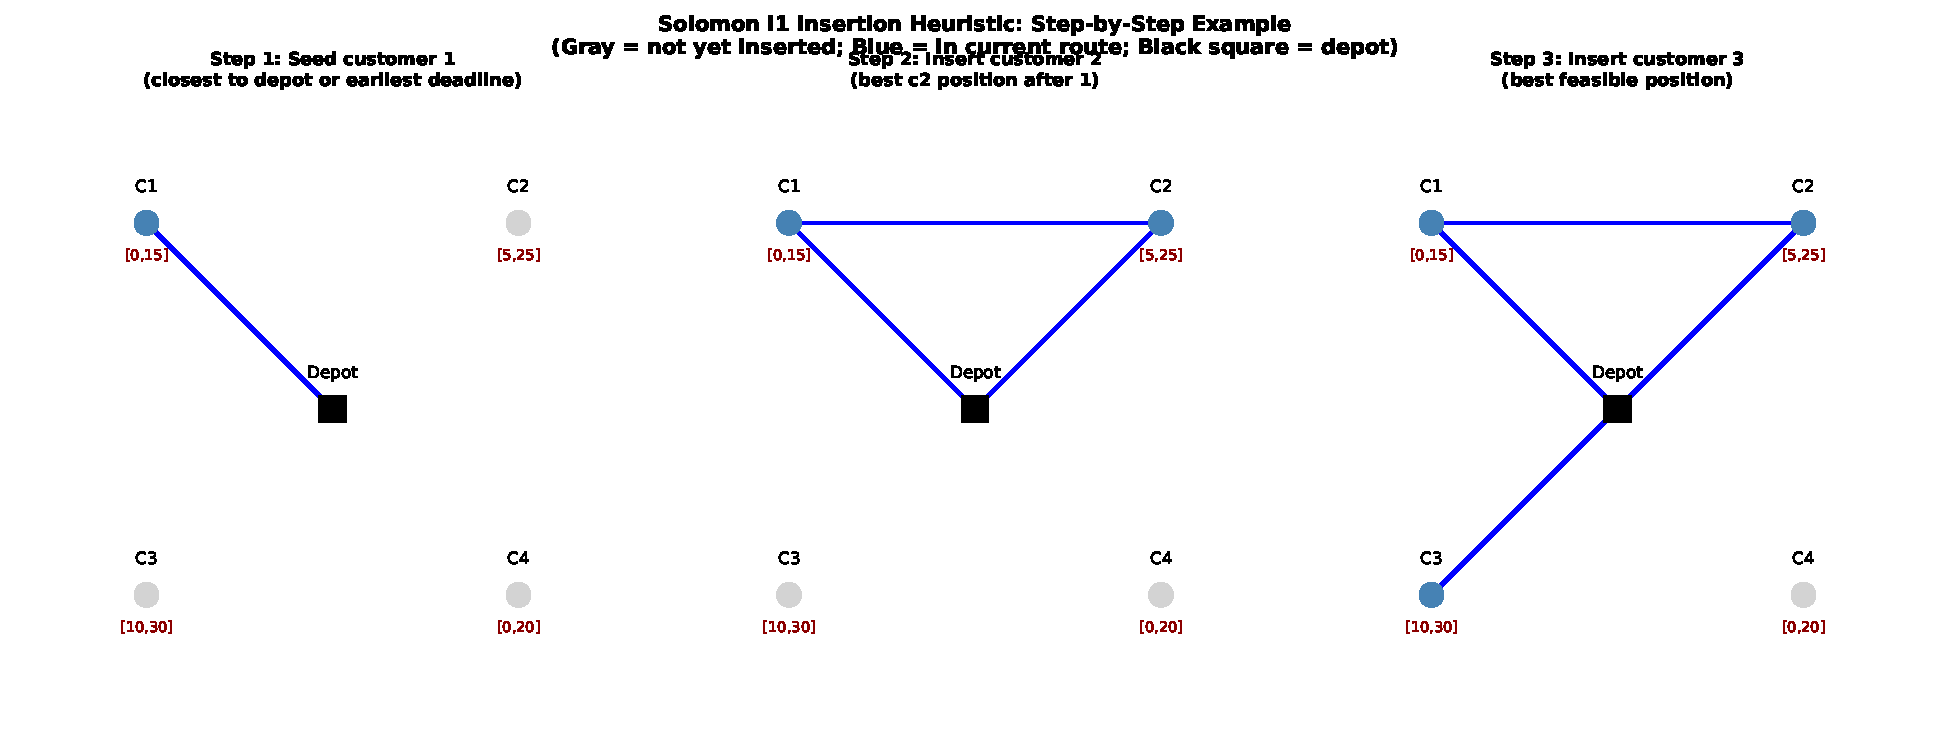
\includegraphics[width=0.85\textwidth]{insertion_heuristic}
  \caption{Three steps of the I1 insertion heuristic on a 4-customer example.
    Grey customers have not yet been inserted; blue customers are on the current
    route.  At each step, the customer with the best $c_2$ score is inserted at
    its cheapest feasible position.}
\end{figure}

\begin{exampleblock}{Worked Numerical Example: I1 with 4 Customers}
Consider 4 customers at positions C1=(2,8), C2=(8,8), C3=(2,2), C4=(8,2),
depot at (5,5).  Time windows: C1=[0,15], C2=[5,25], C3=[10,30], C4=[0,20].
Demands: all = 2; capacity $Q=6$.  Service time $s_i=1$ for all.  Parameters
$\alpha_1=0.5$, $\alpha_2=0.5$, $\lambda=1$.

\textbf{Step 1: Seed.}  Compute $d(\text{depot}, C_i)$: $d_1=\sqrt{9+9}\approx4.24$,
$d_2\approx4.24$, $d_3\approx4.24$, $d_4\approx4.24$ (symmetric; tie broken by
earliest deadline).  Seed: C1 (earliest $b_1=15$).  Route: dep$\to$C1$\to$dep.

\textbf{Step 2: Insert C2.}  Only position is between C1 and depot.
$c_1 = 0.5(d_{C1,C2} + d_{C2,dep} - d_{C1,dep}) + 0.5(b_{C2}^* - b_{dep}^*)$.
$d_{C1,C2}=6$, $d_{C2,dep}=4.24$, $d_{C1,dep}=4.24$.
Extra distance $= 6+4.24-4.24=6$.  Check: $w_{C1}=2, w_{C2}=2+1+6=9\in[5,25]$. Feasible.

\textbf{Step 3:} Continue inserting C4 and C3 into the route or a new route,
always checking capacity $\leq 6$ and time windows.  When inserting C3 into
the current route would violate the capacity (load would become 6), we check if
the time windows still allow it.
\end{exampleblock}

\end{frame}

\begin{frame}[allowframebreaks]{5.4.1 --- Neighbourhood Search Methods}

A \emph{neighbourhood} of a solution $s$ is a set $N(s)$ of solutions reachable
from $s$ by applying a single \emph{move operation}.  Local search starts from a
feasible solution and repeatedly moves to a better neighbour.

\bigskip
\textbf{Intra-route neighbourhoods} (moves within a single route):

\begin{itemize}
  \item \textbf{2-opt:} Remove two arcs $(i, i')$ and $(j, j')$ from the route
    and reconnect the four endpoints by adding arcs $(i,j)$ and $(i',j')$,
    thereby reversing the segment between $i'$ and $j$.  Accept the move if
    the new route is feasible and shorter.
  \item \textbf{Or-opt} (also called \textbf{1-opt} or \textbf{relocation}):
    Move a single customer (or a segment of 2 or 3 consecutive customers) to
    a different position in the same route.
\end{itemize}

\begin{figure}
  \centering
  
\includegraphics[width=0.72\textwidth]{two_opt}
  \caption{The 2-opt move.  Two crossing arcs (dashed red) are replaced by
    two non-crossing arcs.  The segment between the two removed arcs is reversed.
    This always reduces total distance if the arcs were crossing.}
\end{figure}

\framebreak

\textbf{Inter-route neighbourhoods} (moves across two or more routes):

\begin{itemize}
  \item \textbf{Or-opt (inter-route):} Move a customer from one route to a
    different route.  This is the key move for reducing vehicle count.
  \item \textbf{Cross-exchange:} Exchange a segment of consecutive customers
    between two routes.  This can create better temporal alignment when routes
    have complementary time windows.
  \item \textbf{2-opt* (two-opt-star):} A modified 2-opt that swaps the \emph{tails}
    of two routes: all customers from position $p$ onward in route 1 are
    transferred to route 2, and vice versa.  Unlike standard 2-opt, 2-opt* operates
    across routes.
  \item \textbf{Path relocation:} Move a connected segment of $k$ customers (a
    \emph{path}) from one route to another.
\end{itemize}

\begin{figure}
  \centering
  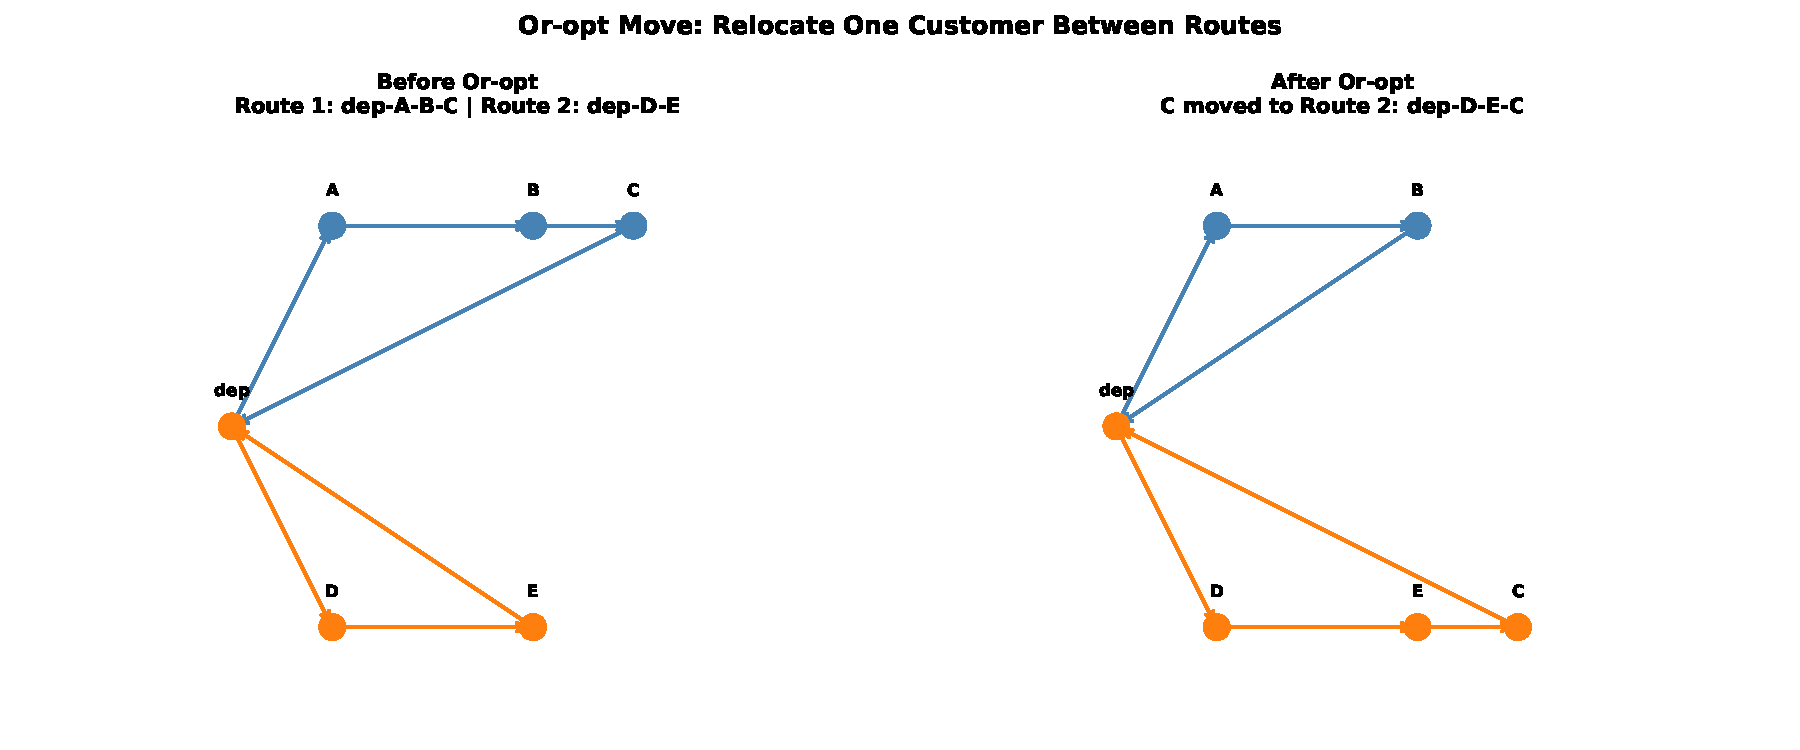
\includegraphics[width=0.68\textwidth]{oropt}
  \caption{Or-opt move: customer C is removed from Route 1 and inserted into
    Route 2.  This reduces Route 1's load and may allow a vehicle to be eliminated.}
\end{figure}

\framebreak

\begin{figure}
  \centering
  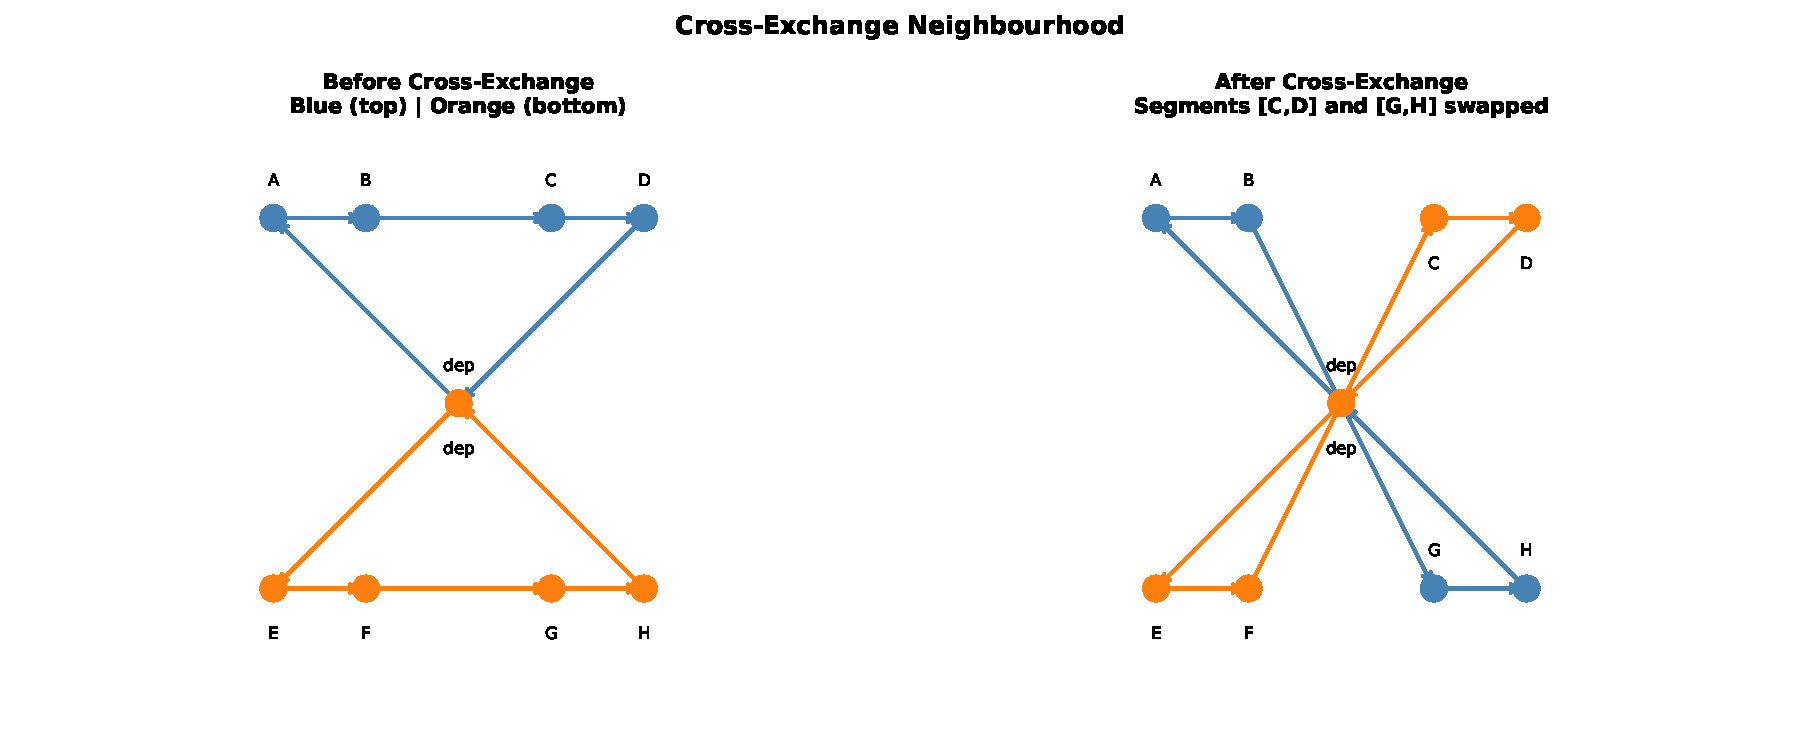
\includegraphics[width=0.72\textwidth]{cross_exchange}
  \caption{Cross-exchange: segment $[C,D]$ from the blue route is swapped with
    segment $[G,H]$ from the orange route.  Both routes must remain feasible after
    the swap (time windows and capacity must still be satisfied).}
\end{figure}

\begin{alertblock}{Key Insight: Time Window Feasibility After Moves}
When performing any neighbourhood move in the VRPTW, all affected routes must be
checked for time-window feasibility after the move.  This is more expensive than
in the pure VRP.  Efficient feasibility checking using \emph{time-window
propagation} (updating arrival times incrementally from the point of modification)
is crucial for practical local search performance.  For a route of $n$ customers,
a naive re-check costs $O(n)$; with proper data structures (e.g., storing earliest
and latest feasible times), many moves can be evaluated in $O(1)$.
\end{alertblock}

\end{frame}

\begin{frame}[allowframebreaks]{5.4.2 --- Single Trajectory Search: Local Search and ILS}

The simplest metaheuristic framework is \textbf{single trajectory search}: at each
step, apply a neighbourhood move and decide whether to accept it.  The decision
rule distinguishes different methods.

\begin{block}{Algorithm 5.1: Large Neighbourhood Search (LNS)}
\begin{algorithmic}[1]
\State $s \leftarrow$ initial feasible solution (e.g., from I1 heuristic)
\State $s^* \leftarrow s$ (best solution found so far)
\Repeat
  \State $s' \leftarrow \text{Destroy}(s)$
    \Comment{Remove a subset of customers from $s$}
  \State $s' \leftarrow \text{Repair}(s')$
    \Comment{Re-insert removed customers into $s'$}
  \If{$f(s') < f(s)$}
    \State $s \leftarrow s'$
  \EndIf
  \If{$f(s') < f(s^*)$}
    \State $s^* \leftarrow s'$
  \EndIf
\Until{stopping criterion (e.g., iteration limit or time limit)}
\State \Return $s^*$
\end{algorithmic}
\end{block}

\framebreak

\textbf{LNS intuition.}  The classical local search neighbourhoods (2-opt, Or-opt)
are \emph{small}: they change only a tiny portion of the solution.  Large
Neighbourhood Search (Shaw 1998) argues that it is more productive to destroy a
large portion of the current solution (removing 10--30 customers simultaneously)
and reconstruct it.  The large destruction step ``unlocks'' the solution from local
minima that small moves cannot escape.

\begin{figure}
  \centering
  
\includegraphics[width=0.85\textwidth]{lns}
  \caption{LNS applied to a 10-customer instance.  Left: initial feasible solution.
    Middle: three customers (C3, C6, C8) are removed (red crosses) in the destroy phase.
    Right: the removed customers are re-inserted using a greedy repair heuristic.
    The repair may produce a different (and hopefully better) assignment.}
\end{figure}

\framebreak

\begin{block}{Adaptive LNS (ALNS)}
Ropke and Pisinger (2006) extended LNS to \textbf{Adaptive LNS (ALNS)}, which
maintains \emph{multiple destroy and repair operators} and adaptively adjusts
the probability of using each operator based on its historical performance.

\medskip
Specifically, each operator $\phi$ (phi, Greek letter) has a weight $w_\phi$.
After each iteration, the weight is updated as:
\[
  w_\phi \leftarrow (1 - r) \cdot w_\phi + r \cdot \sigma_\phi
\]
where $r$ (rho, a reaction parameter) controls how quickly the algorithm adapts,
and $\sigma_\phi$ (sigma sub phi) is a score based on how well operator $\phi$
performed (e.g., $\sigma=3$ if the new solution is a new global best; $\sigma=2$
if it improves the current solution; $\sigma=1$ if it is accepted; $\sigma=0$
otherwise).  The selection probability of operator $\phi$ at each step is
proportional to $w_\phi$.  This is analogous to a multi-armed bandit problem.
\end{block}

\begin{alertblock}{Why ``Adaptive'' Helps}
Different destroy/repair operators work better on different instance types.  For
clustered instances (C1, C2), removing a geographic cluster of customers is
effective; for random instances (R1, R2), a random removal works well.  ALNS
automatically discovers which operators work and allocates more probability to them.
This explains why ALNS consistently outperforms fixed-operator LNS.
\end{alertblock}

\end{frame}

\begin{frame}[allowframebreaks]{5.4.2 --- Iterated Local Search (ILS)}

\textbf{Iterated Local Search (ILS)} is another single-trajectory framework that
applies a \emph{perturbation} to escape local optima.

\begin{block}{ILS for VRPTW}
\begin{algorithmic}[1]
\State $s_0 \leftarrow$ initial solution (e.g., from I1); $s \leftarrow \text{LocalSearch}(s_0)$
\State $s^* \leftarrow s$
\Repeat
  \State $s' \leftarrow \text{Perturb}(s)$
    \Comment{Apply a random large move (e.g., random 3-opt)}
  \State $s'' \leftarrow \text{LocalSearch}(s')$
    \Comment{Re-apply local search from perturbed solution}
  \State $s \leftarrow \text{Accept}(s, s'')$
    \Comment{Accept if better, or by some probabilistic criterion}
  \If{$f(s'') < f(s^*)$}
    \State $s^* \leftarrow s''$
  \EndIf
\Until{stopping criterion}
\State \Return $s^*$
\end{algorithmic}
\end{block}

\textbf{Key idea.}  ILS alternates between deep local search (finding a local
optimum) and perturbation (jumping to a different basin of attraction).  The
perturbation must be strong enough to escape the current basin but not so strong
that it destroys all structure.  For VRPTW, effective perturbations include
random Or-opt moves or random segment cross-exchanges.

\end{frame}

\begin{frame}[allowframebreaks]{5.4.3 --- Population-Based Search: Evolutionary Algorithms}

\textbf{Evolutionary algorithms (EAs)} maintain a \emph{population} of solutions
(rather than a single current solution) and improve them by applying
\emph{selection}, \emph{recombination} (crossover), and \emph{mutation}
(local improvement).

\begin{block}{General EA Framework for VRPTW}
\begin{algorithmic}[1]
\State Generate initial population $P$ of $N$ feasible solutions (using I1 or random)
\Repeat
  \State \textbf{Selection:} Choose two parent solutions $s_a, s_b \in P$
    (e.g., tournament selection)
  \State \textbf{Recombination:} Apply crossover operator to $s_a, s_b$ to
    produce offspring $s'$
  \State \textbf{Improvement:} Apply local search to $s'$ to find local optimum
  \State \textbf{Replacement:} Insert $s'$ into $P$; remove worst individual
    (or apply diversity criterion)
\Until{stopping criterion}
\State \Return best solution in $P$
\end{algorithmic}
\end{block}

\framebreak

\begin{block}{Crossover Operators for VRPTW}
Recombination in VRPTW must produce feasible children.  Two effective operators are:

\begin{itemize}
  \item \textbf{Order Crossover (OX):} Copy a segment of the customer sequence from
    parent $s_a$ into the child; fill the remaining positions with customers from
    parent $s_b$ in their original order.  This preserves the relative ordering of
    customers from both parents.

  \item \textbf{Edge Assembly Crossover (EAX):} Identify arcs that appear in parent
    $s_a$ but not $s_b$ (and vice versa) and systematically reassemble routes using
    those arcs.  EAX tends to preserve more route structure and is particularly
    effective for VRPTW.

  \item \textbf{Split + recombination:} Apply Prins' \emph{split} algorithm:
    represent each solution as a giant tour (all customers in a single sequence),
    apply crossover on the giant tour, then use dynamic programming (split) to
    partition it optimally into routes respecting capacity and time windows.
\end{itemize}
\end{block}

\begin{exampleblock}{EAX on a Small VRPTW Instance}
Parent 1: Route A = [1, 2, 3], Route B = [4, 5].
Parent 2: Route C = [1, 4, 2], Route D = [3, 5].

\medskip
EAX identifies ``AB-cycles'': arcs in Parent 1's routes that form cycles when
composed with Parent 2's arcs.  By selecting which cycles to inherit from each
parent, offspring with novel route combinations are created while preserving
partial sub-sequences from both parents.
\end{exampleblock}

\end{frame}

\begin{frame}[allowframebreaks]{5.4.3 --- Metaheuristic Overview: Tabu Search}

\textbf{Tabu Search (TS)}, introduced by Glover (1986), is one of the most
successful metaheuristics for the VRPTW.  The analogy is this: a problem-solver
exploring a landscape is allowed to ``revisit'' previously seen solutions, but
maintains a \emph{tabu list} of recently visited solutions or moves that are
temporarily forbidden.  This prevents cycling and forces exploration of new areas.

\begin{block}{Tabu Search for VRPTW}
\begin{algorithmic}[1]
\State $s \leftarrow$ initial feasible solution; $s^* \leftarrow s$
\State $\mathcal{T} \leftarrow \emptyset$ (tabu list, length $|\mathcal{T}| = \ell$)
\Repeat
  \State Generate candidate moves $N(s)$ (e.g., all Or-opt, 2-opt* moves)
  \State $s' \leftarrow \arg\min_{s'' \in N(s) \setminus \mathcal{T}} f(s'')$
    \Comment{Best non-tabu move}
  \If{$f(s') < f(s^*)$ (aspiration criterion)}
    \State Accept $s'$ even if tabu; $s^* \leftarrow s'$
  \EndIf
  \State $s \leftarrow s'$
  \State Add move generating $s'$ to $\mathcal{T}$; remove oldest if $|\mathcal{T}| > \ell$
\Until{stopping criterion}
\State \Return $s^*$
\end{algorithmic}
\end{block}

\framebreak

\textbf{Key parameters of Tabu Search:}
\begin{itemize}
  \item \textbf{Tabu list length $\ell$:}  Short lists allow rapid escape from
    local optima but risk cycling; long lists enforce more diversification but
    may prevent beneficial moves.  Dynamic tabu list length (adapted based on
    solution quality) is common.
  \item \textbf{Aspiration criterion:}  A tabu move is permitted if it produces a
    new global best.  This is nearly universal in TS implementations.
  \item \textbf{Diversification:}  After a long period without improvement, reset
    the solution or force exploration of under-visited areas.
  \item \textbf{Infeasibility handling:}  Many VRPTW TS implementations allow
    temporary infeasibility (e.g., slight capacity violations) with a penalty,
    then repair the solution.  This enlarges the neighbourhood and prevents getting
    trapped by feasibility constraints.
\end{itemize}

\begin{figure}
  \centering
  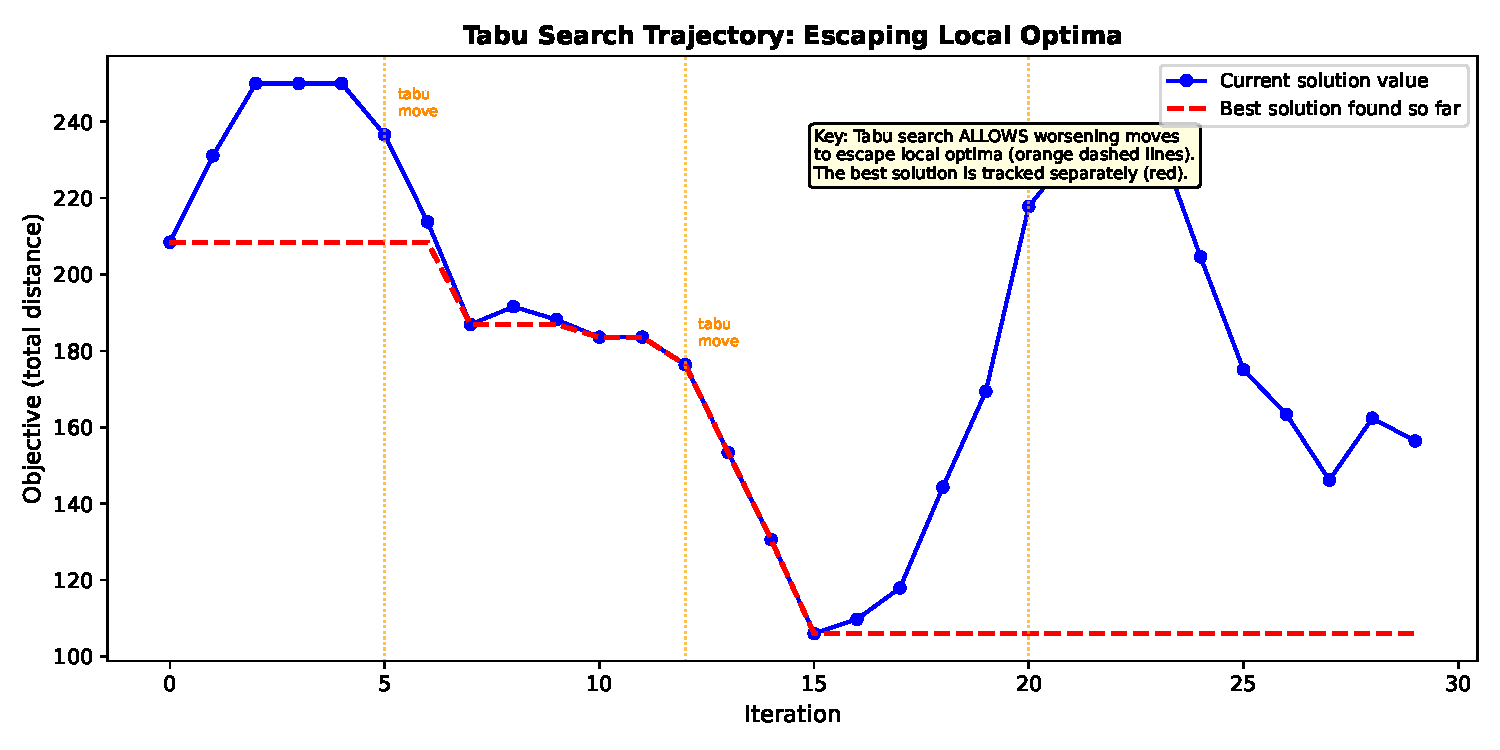
\includegraphics[width=0.70\textwidth]{tabu_trajectory}
  \caption{Tabu search trajectory.  The current solution value (blue) is allowed
    to worsen at tabu moves (orange vertical lines), enabling escape from local
    minima.  The best solution found (red dashed line) monotonically improves.}
\end{figure}

\framebreak

\begin{alertblock}{Allowing Infeasibility in Tabu Search}
A key innovation in VRPTW tabu search (e.g., Taillard et al.\ 1997; Cordeau,
Laporte, Mercier 2001) is to allow \emph{temporarily infeasible} solutions during
search.  Instead of hard constraints on capacity and time windows, violations are
penalised in the objective function.  The algorithm oscillates between feasible
and infeasible regions, achieving much richer exploration.  The penalty weights are
tuned dynamically: if the search has been infeasible for too long, increase
penalties; if it has been overly constrained, reduce them.
\end{alertblock}

\end{frame}

\begin{frame}[allowframebreaks]{5.4.3 --- Simulated Annealing (SA) and Guided Local Search (GLS)}

\textbf{Simulated Annealing (SA).}  The analogy comes from metallurgy: when metal
is slowly cooled (\emph{annealed}), atoms settle into low-energy crystal structures.
Similarly, SA starts with a high ``temperature'' $T$ (theta-like parameter) that
allows accepting worse solutions with high probability, then gradually reduces $T$,
progressively narrowing the search to improve solutions.

\begin{block}{SA Acceptance Rule}
A candidate solution $s'$ (generated by a random neighbourhood move from $s$) is
accepted if:
\[
  f(s') < f(s) \quad \text{(improvement, always accepted)}
  \quad\text{or}\quad
  \text{Uniform}[0,1] < \exp\!\left(\frac{f(s) - f(s')}{T}\right)
\]
Here $T$ is the current temperature.  When $T$ is large, $\exp(\cdot)$ is close to
1 and even large worsening moves are accepted.  As $T \to 0$, the acceptance
probability of worse moves approaches 0 and SA reduces to greedy descent.
\end{block}

\textbf{Cooling schedule:} A common geometric cooling schedule is $T \leftarrow
\beta \cdot T$ after each iteration (where $\beta$ (beta) is slightly less than 1,
e.g., $\beta = 0.9999$).  The initial temperature $T_0$ and final temperature $T_f$
must be tuned carefully.

\framebreak

\textbf{Guided Local Search (GLS).}  Proposed by Voudouris and Tsang (1999), GLS
augments the objective function with penalty terms for features of solutions that
have been visited often without improvement.

\begin{block}{GLS Augmented Objective}
\[
  h(s) = f(s) + \lambda \sum_{i=1}^{m} p_i \cdot I_i(s)
\]
Here $m$ is the number of solution features (e.g., individual arcs), $p_i$ (p sub
$i$) is the penalty for feature $i$ (incremented each time feature $i$ appears in
a local optimum), $I_i(s)$ (indicator sub $i$) equals 1 if feature $i$ is present
in solution $s$, and $\lambda$ (lambda) is the penalty weight.  After reaching each
local optimum of $h$, the penalty of the feature with highest
$\text{utility}_i = I_i(s) \cdot c_i / (1 + p_i)$ is incremented by 1.

\medskip
The key insight is that GLS \emph{remembers} which arcs or sub-routes appear
repeatedly in local optima and penalises them, forcing the search to explore
qualitatively different solutions.  Prins and Bouchenoua (2004) applied GLS
successfully to the VRPTW.
\end{block}

\end{frame}

\begin{frame}[allowframebreaks]{5.4.3 --- Metaheuristic Comparison Table}

The following table summarises the key features of the most important metaheuristics
for the VRPTW, based on Table 5.2 from the book (comparison of published methods).

\begin{center}
\begin{tabular}{llccccc}
\toprule
\textbf{Method} & \textbf{Ref.} & \textbf{2-opt} & \textbf{Or-opt*} & \textbf{Cross} & \textbf{LNS} & \textbf{Vehicle min.} \\
\midrule
SA              & BVH04  & $\times$ & $\times$ & $\times$ &           & $\times$ \\
TS              & MB05   &          &          & $\times$ &           & $\times$ \\
GLS             & PR07   &          &          &          & $\times$  & $\times$ \\
ILS             & HY08   & $\times$ & $\times$ & $\times$ &           &          \\
LNS/CE          & IINSUY08 &       &          &          & $\times$  &          \\
ALNS            & RT09   & $\times$ &          & 3        & $\times$  & $\times$ \\
EA+LNS          & PDR09  &          &          & 3        & $\times$  &          \\
ILS+LNS         & NBD10  & $\times$ & $\times$ & 1        & $\times$  & $\times$ \\
Hybrid          & VCGP13 &          & $\times$ & 2        & $\times$  & $\times$ \\
\bottomrule
\end{tabular}
\end{center}

\begin{figure}
  \centering
  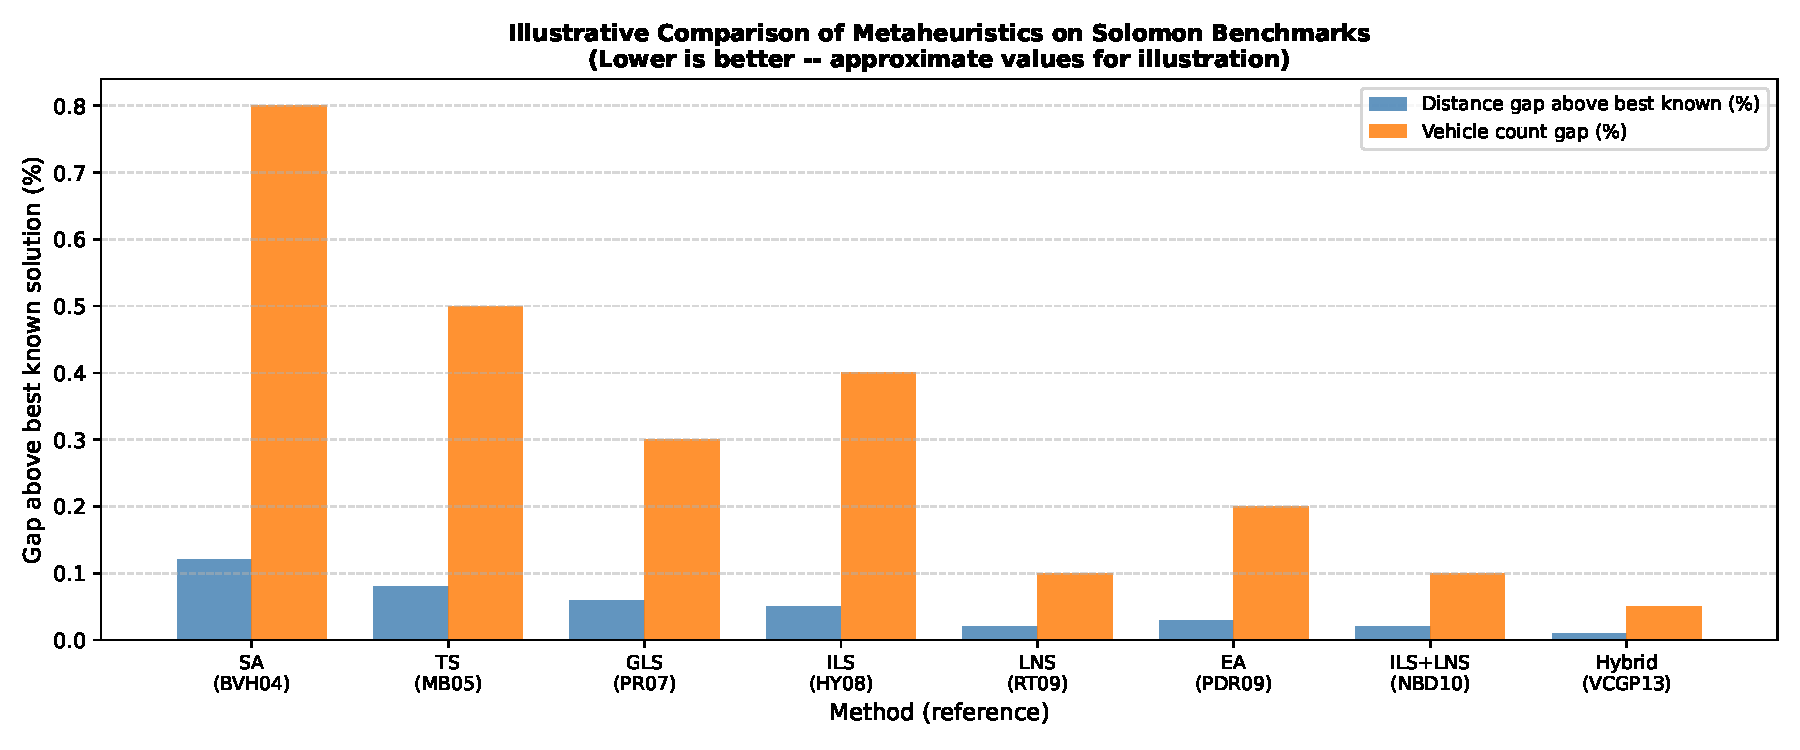
\includegraphics[width=0.72\textwidth]{metaheuristic_comparison}
  \caption{Illustrative comparison of metaheuristic quality on Solomon benchmarks.
    Lower bars indicate smaller gap above the best known solution.  Hybrid methods
    combining multiple neighbourhoods and LNS (right side) consistently achieve the
    smallest gaps.}
\end{figure}

\end{frame}

\begin{frame}[allowframebreaks]{5.5 --- Summary Computational Results for Exact Methods}

Table 5.3 in the book reports results of the best exact Branch-and-Price algorithms
on Solomon instances.  The instances are grouped into two classes:

\begin{itemize}
  \item \textbf{Class 1} (C1, R1, RC1): tight time windows, many vehicles.
  \item \textbf{Class 2} (C2, R2, RC2): wide time windows, few vehicles.
\end{itemize}

\begin{figure}
  \centering
  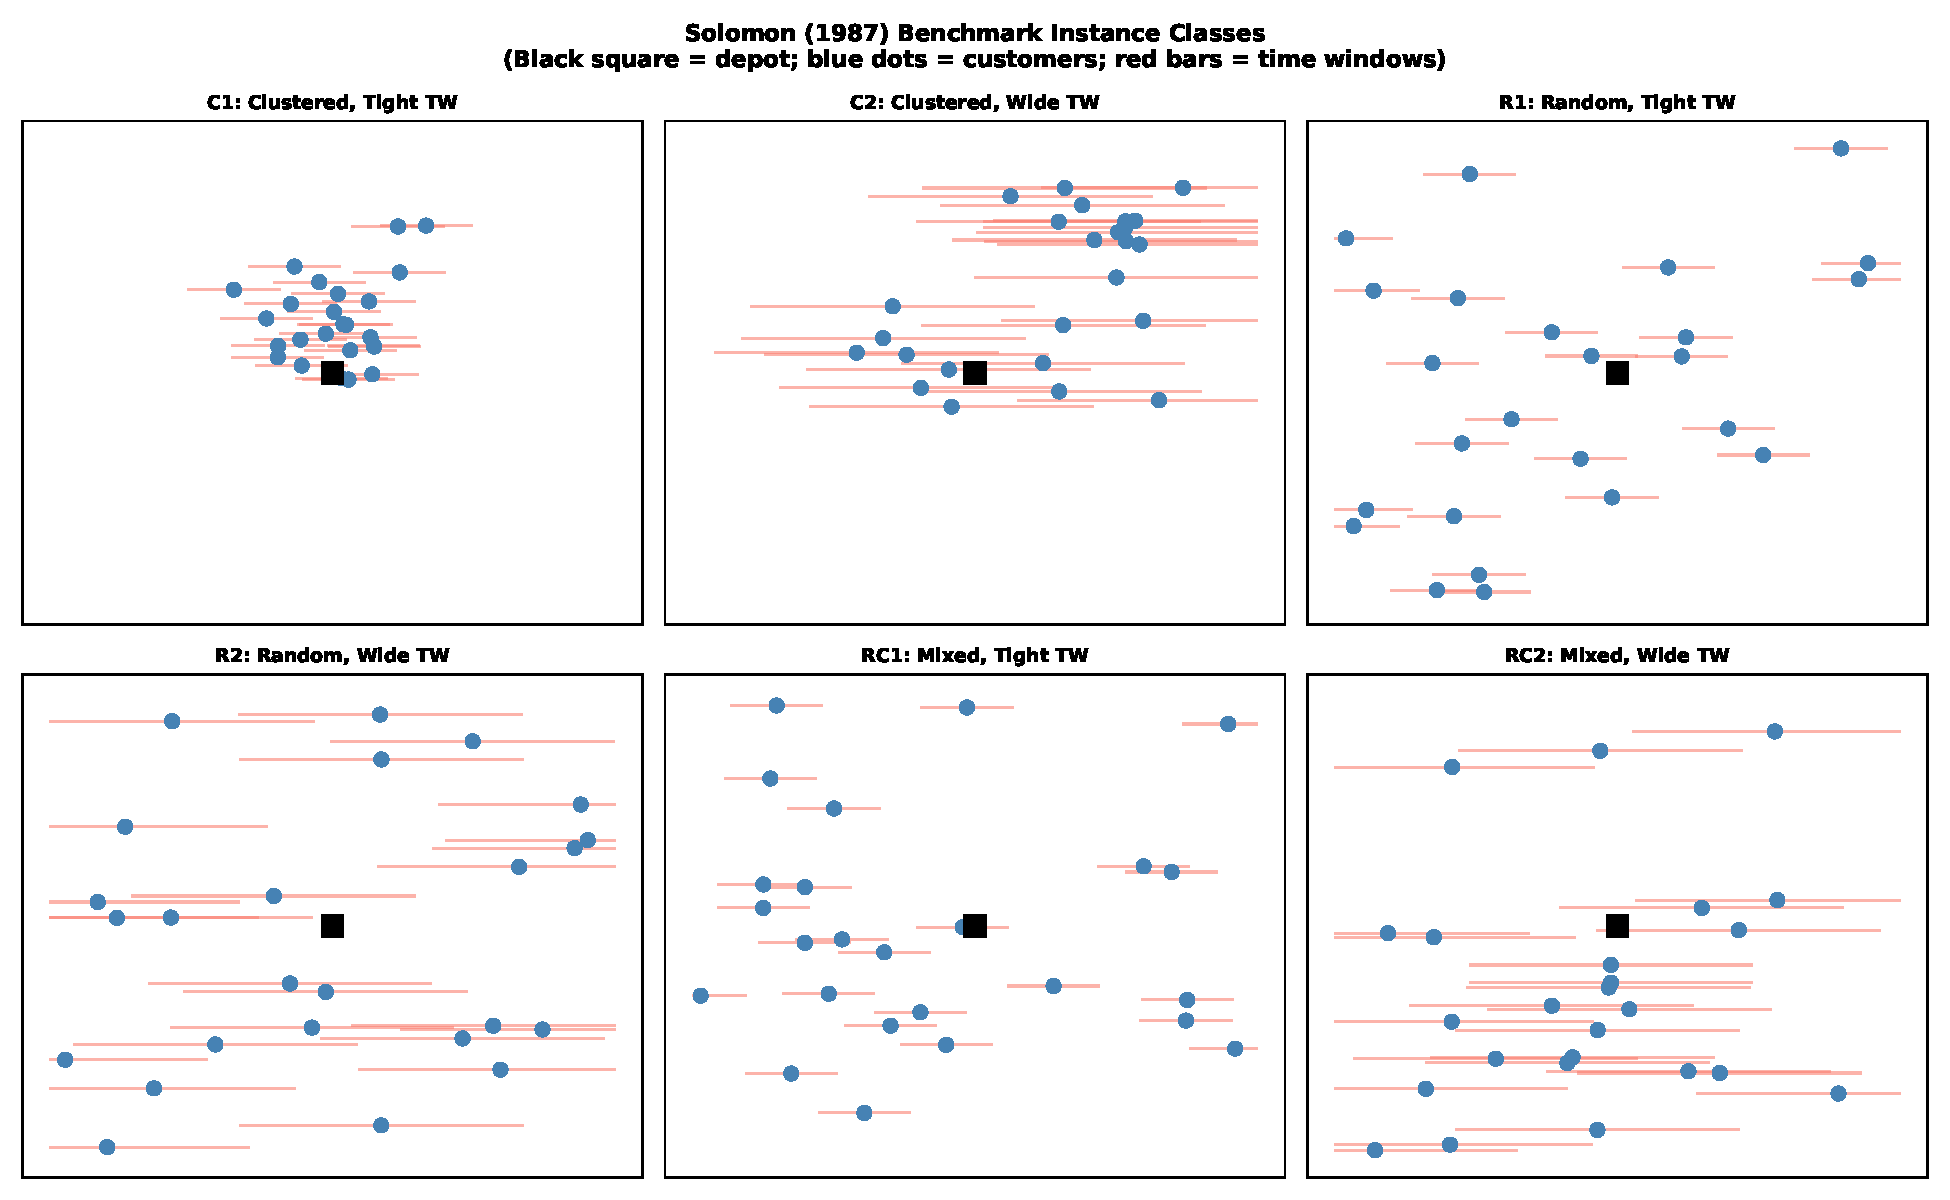
\includegraphics[width=0.72\textwidth]{solomon_instances}
  \caption{Solomon benchmark instance classes.  Clustered instances (C1, C2) have
    customers grouped around centres.  Random instances (R1, R2) distribute
    customers uniformly.  Mixed instances (RC1, RC2) combine both.  Red bars
    illustrate time window widths: tight in class 1, wide in class 2.}
\end{figure}

\framebreak

Key findings from computational experiments (Table 5.3):

\begin{itemize}
  \item \textbf{Class 1 instances} (tight windows): the Branch-and-Price algorithm
    of Desrochers, Desrosiers, Solomon (DDS92) solved all 25 instances optimally.
    Modern B\&P+C methods require only a small fraction of the computation time
    compared to early methods.
  \item \textbf{Class 2 instances} (wide windows): the SPPRC sub-problem is harder
    (fewer dominated labels) and the tree is larger.  However, with dual
    stabilisation and subset-row inequalities, all 25 Solomon instances have been
    solved optimally.
  \item The Chabrier (2006) B\&P algorithm and the Righini-Salani (2006) bidirectional
    labelling are decisive advances.  Matching lower bounds with LNS upper bounds
    confirms optimality.
  \item For instances with 200--400 customers (Gehring and Homberger benchmark),
    exact methods remain too slow; best results come from metaheuristics.
\end{itemize}

\begin{alertblock}{Benchmark Normalisation}
Results are typically reported as CNV (total number of vehicles across all
instances), CD (total travel distance), and CT (CPU time in seconds).  Comparing
algorithms is done on the \emph{same} computing environment; historical comparisons
must account for Moore's Law (computers double in speed roughly every 2 years).
\end{alertblock}

\end{frame}

% ─── Python Code ─────────────────────────────────────────────────────────────
\begin{frame}[fragile]{Python: Solomon I1 Construction Heuristic}
\begin{lstlisting}[language=Python, caption=Solomon I1 insertion heuristic for VRPTW]
import math

def euclidean(p1, p2):
    return math.hypot(p1[0]-p2[0], p1[1]-p2[1])

def i1_vrptw(depot, customers, Q, alpha1=0.5, alpha2=0.5, lam=1.0):
    """
    Solomon I1 heuristic for VRPTW.
    customers: list of dicts with keys x,y,demand,tw_open,tw_close,service_time
    depot: dict with keys x,y,tw_open,tw_close
    Q: vehicle capacity
    Returns list of routes (each route = list of customer indices)
    """
    n = len(customers)
    unrouted = set(range(n))
    routes = []

    while unrouted:
        # Select seed: farthest from depot (or earliest deadline)
        seed = max(unrouted,
                   key=lambda i: euclidean(
                       (depot['x'], depot['y']),
                       (customers[i]['x'], customers[i]['y'])))
        route = [seed]
        unrouted.remove(seed)
        load = customers[seed]['demand']

        # Compute service start times for current route
        def compute_times(route):
            times = [None]*len(route)
            t = depot['tw_open']
            t += euclidean((depot['x'],depot['y']),
                           (customers[route[0]]['x'],customers[route[0]]['y']))
            t = max(t, customers[route[0]]['tw_open'])
            times[0] = t
            for idx in range(1, len(route)):
                prev, cur = route[idx-1], route[idx]
                t = times[idx-1] + customers[prev]['service_time']
                t += euclidean((customers[prev]['x'],customers[prev]['y']),
                               (customers[cur]['x'],customers[cur]['y']))
                t = max(t, customers[cur]['tw_open'])
                times[idx] = t
            return times

        changed = True
        while changed and unrouted:
            changed = False
            best_u, best_pos, best_c2 = None, None, -1e18
            for u in unrouted:
                if load + customers[u]['demand'] > Q:
                    continue
                # Find best insertion position
                best_c1, best_p = 1e18, None
                for pos in range(len(route)+1):
                    r_new = route[:pos] + [u] + route[pos:]
                    times = compute_times(r_new)
                    # Check time window feasibility
                    feasible = all(
                        times[k] <= customers[r_new[k]]['tw_close']
                        for k in range(len(r_new)))
                    if not feasible:
                        continue
                    # Compute c1
                    if pos == 0:
                        prev_node = depot; prev_t = depot['tw_open']
                    else:
                        prev_node = customers[route[pos-1]]
                        prev_t = compute_times(route)[pos-1]
                    # distance extra
                    d_iu = euclidean((prev_node['x'],prev_node['y']),
                                     (customers[u]['x'],customers[u]['y']))
                    if pos < len(route):
                        next_node = customers[route[pos]]
                        d_uj = euclidean((customers[u]['x'],customers[u]['y']),
                                        (next_node['x'],next_node['y']))
                        d_ij = euclidean((prev_node['x'],prev_node['y']),
                                        (next_node['x'],next_node['y']))
                    else:
                        d_uj = euclidean((customers[u]['x'],customers[u]['y']),
                                        (depot['x'],depot['y']))
                        d_ij = euclidean((prev_node['x'],prev_node['y']),
                                        (depot['x'],depot['y']))
                    c1 = alpha1*(d_iu+d_uj-d_ij) + alpha2*(times[pos]-prev_t)
                    if c1 < best_c1:
                        best_c1, best_p = c1, pos
                if best_p is not None:
                    d_depot_u = euclidean((depot['x'],depot['y']),
                                         (customers[u]['x'],customers[u]['y']))
                    c2 = lam*d_depot_u - best_c1
                    if c2 > best_c2:
                        best_c2, best_u, best_pos = c2, u, best_p
            if best_u is not None:
                route.insert(best_pos, best_u)
                load += customers[best_u]['demand']
                unrouted.remove(best_u)
                changed = True
        routes.append(route)
    return routes
\end{lstlisting}
\end{frame}

\begin{frame}[fragile]{Python: 2-opt Improvement for VRPTW Route}
\begin{lstlisting}[language=Python, caption=2-opt local search for a single VRPTW route]
def check_feasibility(route, customers, depot, Q):
    """Check capacity and time window feasibility of a route."""
    load = sum(customers[i]['demand'] for i in route)
    if load > Q:
        return False, None
    times = []
    t = depot['tw_open']
    prev = (depot['x'], depot['y'])
    for idx, c in enumerate(route):
        t += euclidean(prev, (customers[c]['x'], customers[c]['y']))
        if t > customers[c]['tw_close']:
            return False, None
        t = max(t, customers[c]['tw_open'])
        times.append(t)
        t += customers[c]['service_time']
        prev = (customers[c]['x'], customers[c]['y'])
    return True, times

def two_opt(route, customers, depot, Q):
    """Improve a single route by 2-opt moves."""
    improved = True
    best_route = route[:]
    while improved:
        improved = False
        for i in range(1, len(best_route)-1):
            for j in range(i+1, len(best_route)):
                # Reverse segment [i..j]
                new_route = (best_route[:i] +
                             best_route[i:j+1][::-1] +
                             best_route[j+1:])
                feasible, _ = check_feasibility(
                    new_route, customers, depot, Q)
                if feasible:
                    # Compute distance improvement
                    def route_dist(r):
                        d = euclidean((depot['x'],depot['y']),
                                      (customers[r[0]]['x'],customers[r[0]]['y']))
                        for k in range(len(r)-1):
                            d += euclidean(
                                (customers[r[k]]['x'],customers[r[k]]['y']),
                                (customers[r[k+1]]['x'],customers[r[k+1]]['y']))
                        d += euclidean((customers[r[-1]]['x'],
                                        customers[r[-1]]['y']),
                                       (depot['x'],depot['y']))
                        return d
                    if route_dist(new_route) < route_dist(best_route)-1e-6:
                        best_route = new_route
                        improved = True
                        break
            if improved:
                break
    return best_route
\end{lstlisting}
\end{frame}

% ============================================================
\section{Extensions}
% ============================================================

\begin{frame}[allowframebreaks]{5.5 --- Extensions of the VRPTW}

The basic VRPTW has inspired a rich family of extensions that model real-world
logistics problems more faithfully.  This section surveys the most important ones.

\begin{block}{5.5.1 Split Deliveries}
In the standard VRPTW, each customer is visited by exactly one vehicle.  In the
\textbf{Split Delivery VRPTW (SDVRPTW)}, a customer with large demand can be served
by \emph{multiple} vehicles, each delivering a fraction of the total demand.  This
is useful when a customer's demand exceeds a single vehicle's capacity.

\medskip
The SDVRPTW relaxes the integrality of the coverage constraints:
\[
  \sum_{k \in K} \sum_{j \in V} x_{ij}^k \geq 1 \qquad \forall\, i \in V'
\]
(at least one visit, but possibly more).  The total delivery across all visits
must sum to the demand $d_i$.
\end{block}

\begin{figure}
  \centering
  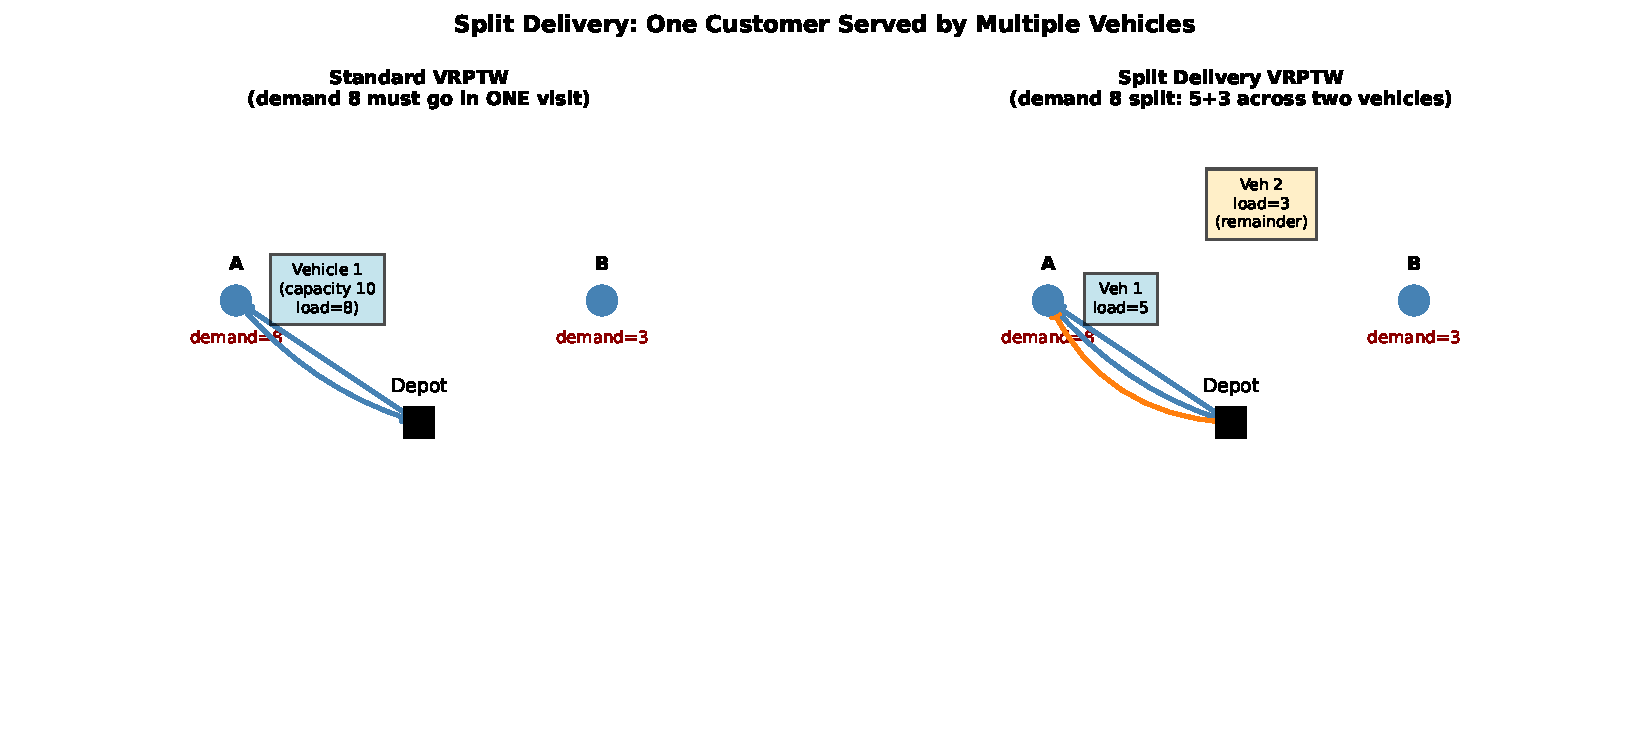
\includegraphics[width=0.72\textwidth]{split_delivery}
  \caption{Split delivery example.  In the standard VRPTW (left), customer A's
    demand of 8 must fit in one vehicle (capacity 10 — just feasible).  In the
    SDVRPTW (right), a second vehicle can deliver the remaining demand, which
    can reduce total route length when the demand makes single-vehicle routing
    awkward.}
\end{figure}

\framebreak

\begin{block}{5.5.2 Time-Dependent Travel Times}
In urban logistics, travel times are not constant: they depend on the time of day
due to traffic congestion.  The \textbf{Time-Dependent VRPTW (TDVRPTW)} replaces
the constant travel time $t_{ij}$ with a function $t_{ij}(\tau)$ (t sub $ij$ of
tau), where $\tau$ (tau, Greek letter) is the departure time from node $i$.

\medskip
The resource extension function for the time resource becomes:
\[
  T_j = \max\bigl(T_i + s_i + t_{ij}(T_i + s_i),\; a_j\bigr)
\]
Notice that $t_{ij}$ now depends on the departure time $T_i + s_i$.  A common
model piecewise-linearly approximates $t_{ij}(\tau)$ using road speed profiles
from historical traffic data (GPS traces, loop detectors).

\medskip
For example, in a metropolitan area, the travel from zone A to zone B takes 10
minutes at 6\,am but 35 minutes during rush hour (8--9\,am).  A route that serves
customer $i$ at 7:50\,am and needs to reach customer $j$ in zone B should plan for
35 minutes, not 10.

The TDVRPTW makes the SPPRC pricing sub-problem harder but remains tractable with
time-discretised arc travel times.
\end{block}

\framebreak

\begin{block}{5.5.3 Multi-Depot VRPTW (MDVRPTW)}
Instead of a single depot, the \textbf{Multi-Depot VRPTW} has $D$ depots.  Each
vehicle is assigned to one depot and must both start and end its route at that
depot.  Customers can potentially be served from any depot.

\medskip
The multi-depot structure complicates both the assignment of customers to depots
and the routing.  A natural formulation replicates the single-depot model with
$D$ origin-destination depot pairs and adds a constraint that each vehicle returns
to its home depot.  The set-partitioning formulation extends cleanly: each feasible
route is now associated with a specific depot, and the column generation
sub-problem (SPPRC) runs separately for each depot.
\end{block}

\begin{block}{5.5.4 Heterogeneous Fleet VRPTW}
In practice, companies operate fleets with vehicles of different capacities,
costs, and speeds.  The \textbf{Heterogeneous Fleet VRPTW (HFVRPTW)} introduces
vehicle types.  Each vehicle type $v$ has its own capacity $Q_v$, fixed cost
$f_v$, and per-unit travel cost $c_{ij}^v$.

\medskip
The three-index formulation extends by indexing binary variables as $x_{ij}^k$
where vehicle $k$ belongs to a specific type.  The column generation approach
separates sub-problems by vehicle type.
\end{block}

\framebreak

\begin{block}{5.5.5 Stochastic VRPTW}
Real logistics operations face uncertainty: demands may be known only in
distribution, travel times may vary, customers may cancel.  The
\textbf{Stochastic VRPTW} models such uncertainty.

\medskip
\textbf{Stochastic demands:} Each customer $i$ has a demand $\tilde{d}_i$ (tilde
$d$ sub $i$) that is a random variable known only in distribution.  A
\emph{two-stage stochastic programming} model plans routes before demands are
realised (first stage) and allows \emph{recourse actions} after realisation
(second stage): if a vehicle's load is exceeded at some customer, it returns to
the depot to reload and resumes the route (at additional cost).

\medskip
The objective minimises expected total cost:
\[
  \min \; c_{\text{routing}} + E[\text{recourse cost}]
\]
where $E[\cdot]$ (E of expectation, the expected value) denotes the expectation
over all demand realisations.

\textbf{Stochastic travel times:} Similarly, $\tilde{t}_{ij}$ is random (e.g.,
Gaussian with mean $\mu_{ij}$ and variance $\sigma_{ij}^2$).  The solution must
be robust: time windows are met with high probability, not just in expectation.
\end{block}

\begin{figure}
  \centering
  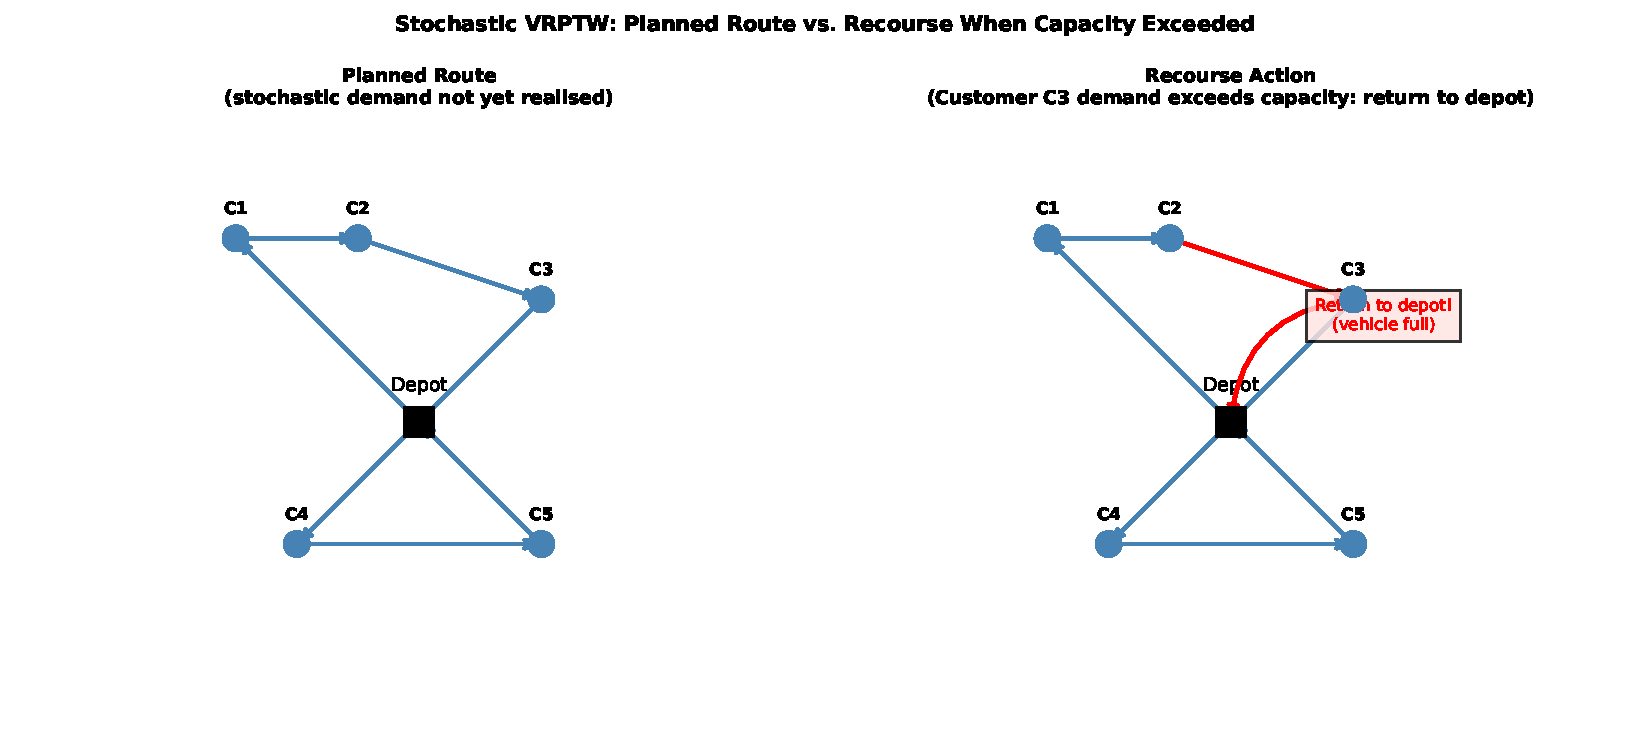
\includegraphics[width=0.72\textwidth]{stochastic_vrptw}
  \caption{Stochastic VRPTW.  The planned route (left) visits customers in a
    fixed sequence.  When customer C3's actual demand exceeds the vehicle's
    remaining capacity, the vehicle returns to the depot (right, red arrow) to
    reload before continuing---a recourse action with additional travel cost.}
\end{figure}

\framebreak

\begin{block}{5.5.6 Driver Considerations and Regulations}
In practice, drivers are subject to legal regulations on driving time and rest
periods (e.g., EU Regulation 561/2006 limits to 9 hours of driving per day).
This adds another resource constraint to the SPPRC:
\begin{itemize}
  \item \textbf{Continuous driving time:} Must not exceed a threshold (e.g., 4.5
    hours) before a mandatory break of at least 45 minutes.
  \item \textbf{Total working time:} Maximum shift length per day.
\end{itemize}
These constraints make the pricing sub-problem harder (more resources) but remain
tractable with multi-dimensional labelling.  Reduced cost fixing becomes more
powerful with more resources (tighter feasibility conditions prune more labels).
\end{block}

\end{frame}

% ============================================================
\section{Conclusions and Future Research Directions}
% ============================================================

\begin{frame}[allowframebreaks]{5.6 --- Conclusions and Future Research}

\textbf{Summary of the chapter.}  The VRPTW is a rich and practically important
optimisation problem that has been the focus of intense research for over three
decades.  The main messages are:

\begin{enumerate}
  \item \textbf{Exact methods.}  Branch-and-Price, powered by column generation
    and the SPPRC, is the state-of-the-art exact approach.  It can solve all 56
    Solomon benchmark instances (100 customers) to optimality.  Key advances
    include bidirectional labelling, dual stabilisation, and valid inequalities
    (subset-row cuts).

  \item \textbf{Heuristics.}  For large instances (200+ customers), metaheuristics
    dominate.  The best-performing methods are hybrid approaches combining large
    neighbourhood search (ALNS) with population-based diversity mechanisms and
    efficient local search.  Differences between top methods are small (within 1\%),
    so the gap between heuristic and optimal is well understood.

  \item \textbf{Benchmarking.}  The Solomon (100-customer) and Gehring-Homberger
    (200--1000 customer) benchmark sets provide universally accepted comparison
    standards.  Best-known solutions are maintained in public repositories.

  \item \textbf{Extensions.}  The VRPTW framework naturally accommodates split
    deliveries, multiple depots, heterogeneous fleets, time-dependent travel,
    stochastic demands, and driver regulations.  Each extension requires adaptations
    to both the formulation and the algorithmic components.
\end{enumerate}

\framebreak

\textbf{Future research directions.}

\begin{itemize}
  \item \textbf{Larger exact instances:}  Current B\&P methods struggle beyond 100
    customers.  Incorporating machine learning to guide branching decisions (e.g.,
    learning variable selection from previous instances) is an active frontier.

  \item \textbf{Rich extensions:}  Combining multiple extensions simultaneously
    (e.g., stochastic + multi-depot + time-dependent) remains largely unsolved
    exactly.  Approximate dynamic programming and robust optimisation approaches
    are promising.

  \item \textbf{Real-time and dynamic VRP:}  Logistics operations are increasingly
    dynamic: orders arrive throughout the day, traffic conditions change in real
    time.  Online algorithms and re-optimisation heuristics are needed.

  \item \textbf{Green VRP with time windows:}  Minimising fuel consumption or
    emissions rather than distance adds a non-linear objective.  Electric vehicle
    routing with charging stops is a particularly active area.

  \item \textbf{Machine learning for heuristics:}  Deep reinforcement learning
    (attention-based models, pointer networks) has shown promise on small VRP
    instances but scaling to VRPTW with 500+ customers remains an open challenge.

  \item \textbf{Parallelism and GPU acceleration:}  Large neighbourhood search
    and population-based methods are embarrassingly parallelisable.  GPU-based
    implementations can evaluate millions of moves per second, potentially enabling
    exact-quality solutions on large instances.
\end{itemize}

\begin{alertblock}{Final Takeaway}
The VRPTW demonstrates how a single, clean mathematical formulation---the
set-partitioning model with column generation---unifies exact and heuristic
methods: column generation solves the LP relaxation, branch-and-price finds integer
solutions, and ALNS achieves near-optimal solutions heuristically.  This
unification of mathematical programming and metaheuristics is one of the great
success stories of modern combinatorial optimisation.
\end{alertblock}

\end{frame}

% ============================================================
\section{Bibliography}
% ============================================================

\begin{frame}[allowframebreaks]{Key References}

\begin{thebibliography}{99}
\small

\bibitem{solomon1987}
  M.~M. Solomon.
  \newblock Algorithms for the vehicle routing and scheduling problems with time
    window constraints.
  \newblock \textit{Operations Research}, 35(2):254--265, 1987.

\bibitem{desrochers1992}
  M.~Desrochers, J.~Desrosiers, and M.~Solomon.
  \newblock A new optimization algorithm for the vehicle routing problem with
    time windows.
  \newblock \textit{Operations Research}, 40(2):342--354, 1992.

\bibitem{dumas1991}
  Y.~Dumas, J.~Desrosiers, and F.~Soumis.
  \newblock The pickup and delivery problem with time windows.
  \newblock \textit{European Journal of Operational Research}, 54(1):7--22, 1991.

\bibitem{righini2006}
  G.~Righini and M.~Salani.
  \newblock Symmetry helps: Bounded bi-directional dynamic programming for the
    elementary shortest path problem with resource constraints.
  \newblock \textit{Discrete Optimization}, 3(3):255--273, 2006.

\bibitem{chabrier2006}
  A.~Chabrier.
  \newblock Vehicle routing problem with elementary shortest path based column
    generation.
  \newblock \textit{Computers \& Operations Research}, 33(10):2972--2990, 2006.

\bibitem{ropke2006}
  S.~Ropke and D.~Pisinger.
  \newblock An adaptive large neighborhood search heuristic for the pickup and
    delivery problem with time windows.
  \newblock \textit{Transportation Science}, 40(4):455--472, 2006.

\bibitem{taillard1997}
  E.~Taillard, P.~Badeau, M.~Gendreau, F.~Guertin, and J.-Y. Potvin.
  \newblock A tabu search heuristic for the vehicle routing problem with soft
    time windows.
  \newblock \textit{Transportation Science}, 31(2):170--186, 1997.

\bibitem{cordeau2001}
  J.-F. Cordeau, G.~Laporte, and A.~Mercier.
  \newblock A unified tabu search heuristic for vehicle routing problems with
    time windows.
  \newblock \textit{Journal of the Operational Research Society}, 52(8):928--936,
    2001.

\bibitem{kallehauge2006}
  B.~Kallehauge, J.~Larsen, O.~B.~G.~Madsen, and M.~M. Solomon.
  \newblock Vehicle routing problem with time windows.
  \newblock In G.~Desaulniers, J.~Desrosiers, and M.~M. Solomon (eds.),
    \textit{Column Generation}, pp.~67--98. Springer, 2005.

\bibitem{rousseau2007}
  L.-M. Rousseau, M.~Gendreau, and D.~Feillet.
  \newblock Interior point stabilization for column generation.
  \newblock \textit{Operations Research Letters}, 35(5):660--668, 2007.

\bibitem{nagata2010}
  Y.~Nagata, O.~Br\"aysy, and W.~Dullaert.
  \newblock A penalty-based edge assembly memetic algorithm for the vehicle
    routing problem with time windows.
  \newblock \textit{Computers \& Operations Research}, 37(4):724--737, 2010.

\bibitem{vidal2013}
  T.~Vidal, T.~G. Crainic, M.~Gendreau, and C.~Prins.
  \newblock A hybrid genetic algorithm with adaptive diversity management for a
    large class of vehicle routing problems with time-windows.
  \newblock \textit{Computers \& Operations Research}, 40(1):475--489, 2013.

\bibitem{shaw1998}
  P.~Shaw.
  \newblock Using constraint programming and local search methods to solve
    vehicle routing problems.
  \newblock In \textit{CP 1998, Lecture Notes in Computer Science}, vol.~1520,
    pp.~417--431. Springer, 1998.

\end{thebibliography}

\end{frame}

% ============================================================
\begin{frame}[allowframebreaks]{End of Chapter 5}
  \begin{center}
    \Large\textbf{Chapter 5: The Vehicle Routing Problem\\with Time Windows}

    \bigskip
    \normalsize
    \textbf{Source:} Desaulniers, Madsen, Ropke (2014).\\
    \textit{Vehicle Routing: Problems, Methods, and Applications}, 2nd ed.\\
    Chapter 5, pp.\ 119--171.

    \bigskip
    \textbf{Key topics covered:}
    \begin{itemize}
      \item VRPTW formulations (three-index, two-index, set-partitioning)
      \item Column generation and Branch-and-Price (SPPRC, labelling)
      \item Construction heuristics (Solomon I1)
      \item Local search neighbourhoods (2-opt, Or-opt, cross-exchange)
      \item Metaheuristics (TS, SA, GLS, LNS/ALNS, ILS, EA)
      \item Extensions: split delivery, time-dependent, multi-depot, stochastic
    \end{itemize}
  \end{center}
\end{frame}

\end{document}
